\documentclass[11pt,compress,t,notes=noshow, aspectratio=169, xcolor=table]{beamer}

\newcommand{\pathiml}{../../slides/06_local-explanations}
\usepackage{../../style/lmu-lecture}
% Defines macros and environments
\usepackage[]{graphicx}
\usepackage[]{color}
% maxwidth is the original width if it is less than linewidth
% otherwise use linewidth (to make sure the graphics do not exceed the margin)
\makeatletter
\def\maxwidth{ %
\ifdim\Gin@nat@width>\linewidth
\linewidth
\else
\Gin@nat@width
\fi
}
\makeatother
%\usepackage[fontsize=10.5pt]{scrextend}
\definecolor{ggred}{rgb}{0.973, 0.463, 0.427}
\definecolor{ggblue}{rgb}{0, 0.749, 0.769}
\definecolor{fgcolor}{rgb}{0.345, 0.345, 0.345}
\newcommand{\hlnum}[1]{\textcolor[rgb]{0.686,0.059,0.569}{#1}}%
\newcommand{\hlstr}[1]{\textcolor[rgb]{0.192,0.494,0.8}{#1}}%
\newcommand{\hlcom}[1]{\textcolor[rgb]{0.678,0.584,0.686}{\textit{#1}}}%
\newcommand{\hlopt}[1]{\textcolor[rgb]{0,0,0}{#1}}%
\newcommand{\hlstd}[1]{\textcolor[rgb]{0.345,0.345,0.345}{#1}}%
\newcommand{\hlkwa}[1]{\textcolor[rgb]{0.161,0.373,0.58}{\textbf{#1}}}%
\newcommand{\hlkwb}[1]{\textcolor[rgb]{0.69,0.353,0.396}{#1}}%
\newcommand{\hlkwc}[1]{\textcolor[rgb]{0.333,0.667,0.333}{#1}}%
\newcommand{\hlkwd}[1]{\textcolor[rgb]{0.737,0.353,0.396}{\textbf{#1}}}%
\newcommand{\predvar}{Var\left[\hat{f}(\xv)\right]}
\let\hlipl\hlkwb

\usepackage{pdfpages}
\usepackage{framed}
\makeatletter
\newenvironment{kframe}{%
\def\at@end@of@kframe{}%
\ifinner\ifhmode%
\def\at@end@of@kframe{\end{minipage}}%
\begin{minipage}{\columnwidth}%
\fi\fi%
\def\FrameCommand##1{\hskip\@totalleftmargin \hskip-\fboxsep
\colorbox{shadecolor}{##1}\hskip-\fboxsep
% There is no \\@totalrightmargin, so:
\hskip-\linewidth \hskip-\@totalleftmargin \hskip\columnwidth}%
\MakeFramed {\advance\hsize-\width
\@totalleftmargin\z@ \linewidth\hsize
\@setminipage}}%
{\par\unskip\endMakeFramed%
\at@end@of@kframe}
\makeatother

\definecolor{shadecolor}{rgb}{.97, .97, .97}
\definecolor{messagecolor}{rgb}{0, 0, 0}
\definecolor{warningcolor}{rgb}{1, 0, 1}
\definecolor{errorcolor}{rgb}{1, 0, 0}
\newenvironment{knitrout}{}{} % an empty environment to be redefined in TeX

\usepackage{alltt}
\newcommand{\SweaveOpts}[1]{}  % do not interfere with LaTeX
\newcommand{\SweaveInput}[1]{} % because they are not real TeX commands
\newcommand{\Sexpr}[1]{}       % will only be parsed by R

\usepackage[english]{babel}
\usepackage[utf8]{inputenc}

\usepackage[export]{adjustbox}
\usepackage{dsfont}
\usepackage{verbatim}
\usepackage{amsmath}
\usepackage{amsfonts}
\usepackage{bm}
\usepackage{csquotes}
\usepackage{multirow}
\usepackage{longtable}
\usepackage{booktabs}
\usepackage{enumerate}
\usepackage[absolute,overlay]{textpos}
\usepackage{psfrag}
\usepackage{algorithm}
\usepackage{algpseudocode}
\usepackage{eqnarray}
\usepackage{arydshln}
\usepackage{tabularx}
\usepackage{placeins}
\usepackage{tikz}
\usepackage{setspace}
\usepackage{colortbl}
\usepackage{mathtools}
\usepackage{wrapfig}
\usepackage{bm}
\usepackage[backend=biber]{biblatex}

\usetikzlibrary{tikzmark, shapes,arrows,automata,positioning,calc,chains,trees,  shadows, decorations.pathreplacing}
\tikzset{
%Define standard arrow tip
>=stealth',
%Define style for boxes
punkt/.style={
rectangle,
rounded corners,
draw=black, very thick,
text width=6.5em,
minimum height=2em,
text centered},
% Define arrow style
pil/.style={
->,
thick,
shorten <=2pt,
shorten >=2pt,}
}

\usepackage{subfig}

\usepackage{bbm}
%\newcommand\hmmax{0}
%\newcommand\bmmax{0}
% basic latex stuff
\newcommand{\pkg}[1]{{\fontseries{b}\selectfont #1}} %fontstyle for R packages
\newcommand{\lz}{\vspace{0.5cm}} %vertical space
\newcommand{\dlz}{\vspace{1cm}} %double vertical space
\newcommand{\oneliner}[1] % Oneliner for important statements
{\begin{block}{}\begin{center}\begin{Large}#1\end{Large}\end{center}\end{block}}

% Latexmath Notation
% math spaces
\ifdefined\N                                                                
\renewcommand{\N}{\mathds{N}} % N, naturals
\else \newcommand{\N}{\mathds{N}} \fi 
\newcommand{\Z}{\mathds{Z}} % Z, integers
\newcommand{\Q}{\mathds{Q}} % Q, rationals
\newcommand{\R}{\mathds{R}} % R, reals
\ifdefined\C 
  \renewcommand{\C}{\mathds{C}} % C, complex
\else \newcommand{\C}{\mathds{C}} \fi
\newcommand{\continuous}{\mathcal{C}} % C, space of continuous functions
\newcommand{\M}{\mathcal{M}} % machine numbers
\newcommand{\epsm}{\epsilon_m} % maximum error

% counting / finite sets
\newcommand{\setzo}{\{0, 1\}} % set 0, 1
\newcommand{\setmp}{\{-1, +1\}} % set -1, 1
\newcommand{\unitint}{[0, 1]} % unit interval

% basic math stuff
\newcommand{\xt}{\tilde x} % x tilde
\newcommand{\argmax}{\operatorname{arg\,max}} % argmax
\newcommand{\argmin}{\operatorname{arg\,min}} % argmin
\newcommand{\argminlim}{\mathop{\mathrm{arg\,min}}\limits} % argmax with limits
\newcommand{\argmaxlim}{\mathop{\mathrm{arg\,max}}\limits} % argmin with limits  
\newcommand{\sign}{\operatorname{sign}} % sign, signum
\newcommand{\I}{\mathbb{I}} % I, indicator
\newcommand{\order}{\mathcal{O}} % O, order
\newcommand{\pd}[2]{\frac{\partial{#1}}{\partial #2}} % partial derivative
\newcommand{\floorlr}[1]{\left\lfloor #1 \right\rfloor} % floor
\newcommand{\ceillr}[1]{\left\lceil #1 \right\rceil} % ceiling

% sums and products
\newcommand{\sumin}{\sum\limits_{i=1}^n} % summation from i=1 to n
\newcommand{\sumim}{\sum\limits_{i=1}^m} % summation from i=1 to m
\newcommand{\sumjn}{\sum\limits_{j=1}^n} % summation from j=1 to p
\newcommand{\sumjp}{\sum\limits_{j=1}^p} % summation from j=1 to p
\newcommand{\sumik}{\sum\limits_{i=1}^k} % summation from i=1 to k
\newcommand{\sumkg}{\sum\limits_{k=1}^g} % summation from k=1 to g
\newcommand{\sumjg}{\sum\limits_{j=1}^g} % summation from j=1 to g
\newcommand{\meanin}{\frac{1}{n} \sum\limits_{i=1}^n} % mean from i=1 to n
\newcommand{\meanim}{\frac{1}{m} \sum\limits_{i=1}^m} % mean from i=1 to n
\newcommand{\meankg}{\frac{1}{g} \sum\limits_{k=1}^g} % mean from k=1 to g
\newcommand{\prodin}{\prod\limits_{i=1}^n} % product from i=1 to n
\newcommand{\prodkg}{\prod\limits_{k=1}^g} % product from k=1 to g
\newcommand{\prodjp}{\prod\limits_{j=1}^p} % product from j=1 to p

% linear algebra
\newcommand{\one}{\boldsymbol{1}} % 1, unitvector
\newcommand{\zero}{\mathbf{0}} % 0-vector
\newcommand{\id}{\boldsymbol{I}} % I, identity
\newcommand{\diag}{\operatorname{diag}} % diag, diagonal
\newcommand{\trace}{\operatorname{tr}} % tr, trace
\newcommand{\spn}{\operatorname{span}} % span
\newcommand{\scp}[2]{\left\langle #1, #2 \right\rangle} % <.,.>, scalarproduct
\newcommand{\mat}[1]{\begin{pmatrix} #1 \end{pmatrix}} % short pmatrix command
\newcommand{\Amat}{\mathbf{A}} % matrix A
\newcommand{\Deltab}{\mathbf{\Delta}} % error term for vectors

% basic probability + stats
\renewcommand{\P}{\mathds{P}} % P, probability
\newcommand{\E}{\mathds{E}} % E, expectation
\newcommand{\var}{\mathsf{Var}} % Var, variance
\newcommand{\cov}{\mathsf{Cov}} % Cov, covariance
\newcommand{\corr}{\mathsf{Corr}} % Corr, correlation
\newcommand{\normal}{\mathcal{N}} % N of the normal distribution
\newcommand{\iid}{\overset{i.i.d}{\sim}} % dist with i.i.d superscript
\newcommand{\distas}[1]{\overset{#1}{\sim}} % ... is distributed as ...

% machine learning
\newcommand{\Xspace}{\mathcal{X}} % X, input space
\newcommand{\Yspace}{\mathcal{Y}} % Y, output space
\newcommand{\nset}{\{1, \ldots, n\}} % set from 1 to n
\newcommand{\pset}{\{1, \ldots, p\}} % set from 1 to p
\newcommand{\gset}{\{1, \ldots, g\}} % set from 1 to g
\newcommand{\Pxy}{\mathbb{P}_{xy}} % P_xy
\newcommand{\Exy}{\mathbb{E}_{xy}} % E_xy: Expectation over random variables xy
\newcommand{\xv}{\mathbf{x}} % vector x (bold)
\newcommand{\xtil}{\tilde{\mathbf{x}}} % vector x-tilde (bold)
\newcommand{\yv}{\mathbf{y}} % vector y (bold)
\newcommand{\xy}{(\xv, y)} % observation (x, y)
\newcommand{\xvec}{\left(x_1, \ldots, x_p\right)^\top} % (x1, ..., xp) 
\newcommand{\Xmat}{\mathbf{X}} % Design matrix
\newcommand{\allDatasets}{\mathds{D}} % The set of all datasets
\newcommand{\allDatasetsn}{\mathds{D}_n}  % The set of all datasets of size n 
\newcommand{\D}{\mathcal{D}} % D, data
\newcommand{\Dn}{\D_n} % D_n, data of size n
\newcommand{\Dtrain}{\mathcal{D}_{\text{train}}} % D_train, training set
\newcommand{\Dtest}{\mathcal{D}_{\text{test}}} % D_test, test set
\newcommand{\xyi}[1][i]{\left(\xv^{(#1)}, y^{(#1)}\right)} % (x^i, y^i), i-th observation
\newcommand{\Dset}{\left( \xyi[1], \ldots, \xyi[n]\right)} % {(x1,y1)), ..., (xn,yn)}, data
\newcommand{\defAllDatasetsn}{(\Xspace \times \Yspace)^n} % Def. of the set of all datasets of size n 
\newcommand{\defAllDatasets}{\bigcup_{n \in \N}(\Xspace \times \Yspace)^n} % Def. of the set of all datasets 
\newcommand{\xdat}{\left\{ \xv^{(1)}, \ldots, \xv^{(n)}\right\}} % {x1, ..., xn}, input data
\newcommand{\ydat}{\left\{ \yv^{(1)}, \ldots, \yv^{(n)}\right\}} % {y1, ..., yn}, input data
\newcommand{\yvec}{\left(y^{(1)}, \hdots, y^{(n)}\right)^\top} % (y1, ..., yn), vector of outcomes
\renewcommand{\xi}[1][i]{\xv^{(#1)}} % x^i, i-th observed value of x
\newcommand{\yi}[1][i]{y^{(#1)}} % y^i, i-th observed value of y 
\newcommand{\xivec}{\left(x^{(i)}_1, \ldots, x^{(i)}_p\right)^\top} % (x1^i, ..., xp^i), i-th observation vector
\newcommand{\xj}{\xv_j} % x_j, j-th feature
\newcommand{\xjvec}{\left(x^{(1)}_j, \ldots, x^{(n)}_j\right)^\top} % (x^1_j, ..., x^n_j), j-th feature vector
\newcommand{\phiv}{\mathbf{\phi}} % Basis transformation function phi
\newcommand{\phixi}{\mathbf{\phi}^{(i)}} % Basis transformation of xi: phi^i := phi(xi)

%%%%%% ml - models general
\newcommand{\lamv}{\bm{\lambda}} % lambda vector, hyperconfiguration vector
\newcommand{\Lam}{\bm{\Lambda}}	 % Lambda, space of all hpos
% Inducer / Inducing algorithm
\newcommand{\preimageInducer}{\left(\defAllDatasets\right)\times\Lam} % Set of all datasets times the hyperparameter space
\newcommand{\preimageInducerShort}{\allDatasets\times\Lam} % Set of all datasets times the hyperparameter space
% Inducer / Inducing algorithm
\newcommand{\ind}{\mathcal{I}} % Inducer, inducing algorithm, learning algorithm 

% continuous prediction function f
\newcommand{\ftrue}{f_{\text{true}}}  % True underlying function (if a statistical model is assumed)
\newcommand{\ftruex}{\ftrue(\xv)} % True underlying function (if a statistical model is assumed)
\newcommand{\fx}{f(\xv)} % f(x), continuous prediction function
\newcommand{\fdomains}{f: \Xspace \rightarrow \R^g} % f with domain and co-domain
\newcommand{\Hspace}{\mathcal{H}} % hypothesis space where f is from
\newcommand{\fbayes}{f^{\ast}} % Bayes-optimal model
\newcommand{\fxbayes}{f^{\ast}(\xv)} % Bayes-optimal model
\newcommand{\fkx}[1][k]{f_{#1}(\xv)} % f_j(x), discriminant component function
\newcommand{\fh}{\hat{f}} % f hat, estimated prediction function
\newcommand{\fxh}{\fh(\xv)} % fhat(x)
\newcommand{\fxt}{f(\xv ~|~ \thetab)} % f(x | theta)
\newcommand{\fxi}{f\left(\xv^{(i)}\right)} % f(x^(i))
\newcommand{\fxih}{\hat{f}\left(\xv^{(i)}\right)} % f(x^(i))
\newcommand{\fxit}{f\left(\xv^{(i)} ~|~ \thetab\right)} % f(x^(i) | theta)
\newcommand{\fhD}{\fh_{\D}} % fhat_D, estimate of f based on D
\newcommand{\fhDtrain}{\fh_{\Dtrain}} % fhat_Dtrain, estimate of f based on D
\newcommand{\fhDnlam}{\fh_{\Dn, \lamv}} %model learned on Dn with hp lambda
\newcommand{\fhDlam}{\fh_{\D, \lamv}} %model learned on D with hp lambda
\newcommand{\fhDnlams}{\fh_{\Dn, \lamv^\ast}} %model learned on Dn with optimal hp lambda 
\newcommand{\fhDlams}{\fh_{\D, \lamv^\ast}} %model learned on D with optimal hp lambda 

% discrete prediction function h
\newcommand{\hx}{h(\xv)} % h(x), discrete prediction function
\newcommand{\hh}{\hat{h}} % h hat
\newcommand{\hxh}{\hat{h}(\xv)} % hhat(x)
\newcommand{\hxt}{h(\xv | \thetab)} % h(x | theta)
\newcommand{\hxi}{h\left(\xi\right)} % h(x^(i))
\newcommand{\hxit}{h\left(\xi ~|~ \thetab\right)} % h(x^(i) | theta)
\newcommand{\hbayes}{h^{\ast}} % Bayes-optimal classification model
\newcommand{\hxbayes}{h^{\ast}(\xv)} % Bayes-optimal classification model

% yhat
\newcommand{\yh}{\hat{y}} % yhat for prediction of target
\newcommand{\yih}{\hat{y}^{(i)}} % yhat^(i) for prediction of ith targiet
\newcommand{\resi}{\yi- \yih}

% theta
\newcommand{\thetah}{\hat{\theta}} % theta hat
\newcommand{\thetab}{\bm{\theta}} % theta vector
\newcommand{\thetabh}{\bm{\hat\theta}} % theta vector hat
\newcommand{\thetat}[1][t]{\thetab^{[#1]}} % theta^[t] in optimization
\newcommand{\thetatn}[1][t]{\thetab^{[#1 +1]}} % theta^[t+1] in optimization
\newcommand{\thetahDnlam}{\thetabh_{\Dn, \lamv}} %theta learned on Dn with hp lambda
\newcommand{\thetahDlam}{\thetabh_{\D, \lamv}} %theta learned on D with hp lambda
\newcommand{\mint}{\min_{\thetab \in \Theta}} % min problem theta
\newcommand{\argmint}{\argmin_{\thetab \in \Theta}} % argmin theta

% densities + probabilities
% pdf of x 
\newcommand{\pdf}{p} % p
\newcommand{\pdfx}{p(\xv)} % p(x)
\newcommand{\pixt}{\pi(\xv~|~ \thetab)} % pi(x|theta), pdf of x given theta
\newcommand{\pixit}[1][i]{\pi\left(\xi[#1] ~|~ \thetab\right)} % pi(x^i|theta), pdf of x given theta
\newcommand{\pixii}[1][i]{\pi\left(\xi[#1]\right)} % pi(x^i), pdf of i-th x 

% pdf of (x, y)
\newcommand{\pdfxy}{p(\xv,y)} % p(x, y)
\newcommand{\pdfxyt}{p(\xv, y ~|~ \thetab)} % p(x, y | theta)
\newcommand{\pdfxyit}{p\left(\xi, \yi ~|~ \thetab\right)} % p(x^(i), y^(i) | theta)

% pdf of x given y
\newcommand{\pdfxyk}[1][k]{p(\xv | y= #1)} % p(x | y = k)
\newcommand{\lpdfxyk}[1][k]{\log p(\xv | y= #1)} % log p(x | y = k)
\newcommand{\pdfxiyk}[1][k]{p\left(\xi | y= #1 \right)} % p(x^i | y = k)

% prior probabilities
\newcommand{\pik}[1][k]{\pi_{#1}} % pi_k, prior
\newcommand{\lpik}[1][k]{\log \pi_{#1}} % log pi_k, log of the prior
\newcommand{\pit}{\pi(\thetab)} % Prior probability of parameter theta

% posterior probabilities
\newcommand{\post}{\P(y = 1 ~|~ \xv)} % P(y = 1 | x), post. prob for y=1
\newcommand{\postk}[1][k]{\P(y = #1 ~|~ \xv)} % P(y = k | y), post. prob for y=k
\newcommand{\pidomains}{\pi: \Xspace \rightarrow \unitint} % pi with domain and co-domain
\newcommand{\pibayes}{\pi^{\ast}} % Bayes-optimal classification model
\newcommand{\pixbayes}{\pi^{\ast}(\xv)} % Bayes-optimal classification model
\newcommand{\pix}{\pi(\xv)} % pi(x), P(y = 1 | x)
\newcommand{\piv}{\bm{\pi}} % pi, bold, as vector
\newcommand{\pikx}[1][k]{\pi_{#1}(\xv)} % pi_k(x), P(y = k | x)
\newcommand{\pikxt}[1][k]{\pi_{#1}(\xv ~|~ \thetab)} % pi_k(x | theta), P(y = k | x, theta)
\newcommand{\pixh}{\hat \pi(\xv)} % pi(x) hat, P(y = 1 | x) hat
\newcommand{\pikxh}[1][k]{\hat \pi_{#1}(\xv)} % pi_k(x) hat, P(y = k | x) hat
\newcommand{\pixih}{\hat \pi(\xi)} % pi(x^(i)) with hat
\newcommand{\pikxih}[1][k]{\hat \pi_{#1}(\xi)} % pi_k(x^(i)) with hat
\newcommand{\pdfygxt}{p(y ~|~\xv, \thetab)} % p(y | x, theta)
\newcommand{\pdfyigxit}{p\left(\yi ~|~\xi, \thetab\right)} % p(y^i |x^i, theta)
\newcommand{\lpdfygxt}{\log \pdfygxt } % log p(y | x, theta)
\newcommand{\lpdfyigxit}{\log \pdfyigxit} % log p(y^i |x^i, theta)

% probababilistic
\newcommand{\bayesrulek}[1][k]{\frac{\P(\xv | y= #1) \P(y= #1)}{\P(\xv)}} % Bayes rule
\newcommand{\muk}{\bm{\mu_k}} % mean vector of class-k Gaussian (discr analysis) 

% residual and margin
\newcommand{\eps}{\epsilon} % residual, stochastic
\newcommand{\epsi}{\epsilon^{(i)}} % epsilon^i, residual, stochastic
\newcommand{\epsh}{\hat{\epsilon}} % residual, estimated
\newcommand{\yf}{y \fx} % y f(x), margin
\newcommand{\yfi}{\yi \fxi} % y^i f(x^i), margin
\newcommand{\Sigmah}{\hat \Sigma} % estimated covariance matrix
\newcommand{\Sigmahj}{\hat \Sigma_j} % estimated covariance matrix for the j-th class

% ml - loss, risk, likelihood
\newcommand{\Lyf}{L\left(y, f\right)} % L(y, f), loss function
\newcommand{\Lypi}{L\left(y, \pi\right)} % L(y, pi), loss function
\newcommand{\Lxy}{L\left(y, \fx\right)} % L(y, f(x)), loss function
\newcommand{\Lxyi}{L\left(\yi, \fxi\right)} % loss of observation
\newcommand{\Lxyt}{L\left(y, \fxt\right)} % loss with f parameterized
\newcommand{\Lxyit}{L\left(\yi, \fxit\right)} % loss of observation with f parameterized
\newcommand{\Lxym}{L\left(\yi, f\left(\bm{\tilde{x}}^{(i)} ~|~ \thetab\right)\right)} % loss of observation with f parameterized
\newcommand{\Lpixy}{L\left(y, \pix\right)} % loss in classification
\newcommand{\Lpiv}{L\left(y, \piv\right)} % loss in classification
\newcommand{\Lpixyi}{L\left(\yi, \pixii\right)} % loss of observation in classification
\newcommand{\Lpixyt}{L\left(y, \pixt\right)} % loss with pi parameterized
\newcommand{\Lpixyit}{L\left(\yi, \pixit\right)} % loss of observation with pi parameterized
\newcommand{\Lhxy}{L\left(y, \hx\right)} % L(y, h(x)), loss function on discrete classes
\newcommand{\Lr}{L\left(r\right)} % L(r), loss defined on residual (reg) / margin (classif)
\newcommand{\lone}{|y - \fx|} % L1 loss
\newcommand{\ltwo}{\left(y - \fx\right)^2} % L2 loss
\newcommand{\lbernoullimp}{\ln(1 + \exp(-y \cdot \fx))} % Bernoulli loss for -1, +1 encoding
\newcommand{\lbernoullizo}{- y \cdot \fx + \log(1 + \exp(\fx))} % Bernoulli loss for 0, 1 encoding
\newcommand{\lcrossent}{- y \log \left(\pix\right) - (1 - y) \log \left(1 - \pix\right)} % cross-entropy loss
\newcommand{\lbrier}{\left(\pix - y \right)^2} % Brier score
\newcommand{\risk}{\mathcal{R}} % R, risk
\newcommand{\riskbayes}{\mathcal{R}^\ast}
\newcommand{\riskf}{\risk(f)} % R(f), risk
\newcommand{\riskdef}{\E_{y|\xv}\left(\Lxy \right)} % risk def (expected loss)
\newcommand{\riskt}{\mathcal{R}(\thetab)} % R(theta), risk
\newcommand{\riske}{\mathcal{R}_{\text{emp}}} % R_emp, empirical risk w/o factor 1 / n
\newcommand{\riskeb}{\bar{\mathcal{R}}_{\text{emp}}} % R_emp, empirical risk w/ factor 1 / n
\newcommand{\riskef}{\riske(f)} % R_emp(f)
\newcommand{\risket}{\mathcal{R}_{\text{emp}}(\thetab)} % R_emp(theta)
\newcommand{\riskr}{\mathcal{R}_{\text{reg}}} % R_reg, regularized risk
\newcommand{\riskrt}{\mathcal{R}_{\text{reg}}(\thetab)} % R_reg(theta)
\newcommand{\riskrf}{\riskr(f)} % R_reg(f)
\newcommand{\riskrth}{\hat{\mathcal{R}}_{\text{reg}}(\thetab)} % hat R_reg(theta)
\newcommand{\risketh}{\hat{\mathcal{R}}_{\text{emp}}(\thetab)} % hat R_emp(theta)
\newcommand{\LL}{\mathcal{L}} % L, likelihood
\newcommand{\LLt}{\mathcal{L}(\thetab)} % L(theta), likelihood
\newcommand{\LLtx}{\mathcal{L}(\thetab | \xv)} % L(theta|x), likelihood
\newcommand{\logl}{\ell} % l, log-likelihood
\newcommand{\loglt}{\logl(\thetab)} % l(theta), log-likelihood
\newcommand{\logltx}{\logl(\thetab | \xv)} % l(theta|x), log-likelihood
\newcommand{\errtrain}{\text{err}_{\text{train}}} % training error
\newcommand{\errtest}{\text{err}_{\text{test}}} % test error
\newcommand{\errexp}{\overline{\text{err}_{\text{test}}}} % avg training error

% lm
\newcommand{\thx}{\thetab^\top \xv} % linear model
\newcommand{\olsest}{(\Xmat^\top \Xmat)^{-1} \Xmat^\top \yv} % OLS estimator in LM 

%%%%%% perturbed data
\usepackage{xifthen}
\newcommand{\pert}[3]{\ifthenelse{\equal{#2}{}}{\tilde{#1}}{\ifthenelse{\equal{#3}{}}{\tilde{#1}^{#2}}{\tilde{#1}^{#2|#3}}}}	% command to express that for #1 the subset #2 was perturbed given subset #3

%%%%%% marginalized functions
\newcommand{\fj}{f_j} % marginal function f_j, depending on feature j
\newcommand{\fnj}{f_{-j}} % marginal function f_{-j}, depending on all features but j
\newcommand{\fS}{f_S} % marginal function f_S depending on feature set S
\newcommand{\fnj}{f_{-S}} % marginal function f_{-S}, depending on all features but features in S
\newcommand{\fC}{f_C} % marginal function f_C depending on feature set C
\newcommand{\fhj}{\fh_j} % marginal function fh_j, depending on feature j
\newcommand{\fhnj}{\fh_{-j}} % marginal function fh_{-j}, depending on all features but j
\newcommand{\fhS}{\fh_S} % marginal function fh_S depending on feature set S
\newcommand{\fhnS}{\fh_{-S}} % marginal function fh_{-S}, depending on all features but features in S
\newcommand{\fhC}{\fh_C} % marginal function fh_C depending on feature set C
\newcommand{\XSmat}{\Xmat_S} % Design matrix subset
\newcommand{\XnSmat}{\Xmat__{-S}} % Design matrix subset without S
\newcommand{\XCmat}{\Xmat_C} % Design matrix subset
\newcommand{\Xnj}{\Xmat_{-j}} % Design matrix subset -j = {1, .., j-1, j+1, ..., p}

%%%%% Shapley values
\newcommand{\Scupj}{S \cup \{j\}} % coalition S but without player j
\newcommand{\Scupk}{S \cup \{k\}} % coalition S but without player k
\newcommand{\SsubP}{S \subseteq P} % coalition S subset of P
\newcommand{\SsubPnoj}{\SsubP \setminus \{j\}} % coalition S subset of P without player j
\newcommand{\SsubPnojk}{\SsubP \setminus \{j,k\}} % coalition S subset of P without player k
\newcommand{\phiij}{\hat{\phi}_j^{(i)}} % Shapley value for feature j and observation i

%%%%% LIME 
\newcommand{\Gspace}{\mathcal{G}} % Hypothesis space for surrogate model
\newcommand{\neigh}{\phi_{\xv}} % Proximity measure
\newcommand{\zv}{\mathbf{z}} % Sampled datapoints for surrogate
\newcommand{\Zspace}{\mathcal{Z}} % Space of sampled datapoints
\newcommand{\Gower}{d_G} % Gower distance


\newcommand{\indep}{\perp}
\newcommand{\Ind}{\mathcal{I}}

%new environments
\newenvironment{vbframe}  %frame with breaks and verbatim
{
\begin{frame}%[containsverbatim,allowframebreaks]
}
{
\end{frame}
}

% \newenvironment{vframe}  %frame with verbatim without breaks (to avoid numbering one slided frames)
% {
%  \begin{frame}[containsverbatim]
% }
% {
% \end{frame}
% }

\newenvironment{blocki}[1]   % itemize block
{
 \begin{block}{#1}\begin{itemize}
}
{
\end{itemize}\end{block}
}

\newenvironment{fragileframe}[2]{  %fragile frame with framebreaks
\begin{frame}[allowframebreaks, fragile, environment = fragileframe]
\frametitle{#1}
#2}
{\end{frame}}


\newcommand{\myframe}[2]{  %short for frame with framebreaks
\begin{frame}[allowframebreaks]
\frametitle{#1}
#2
\end{frame}}

\newcommand{\remark}[1]{
  \textbf{Remark:} #1
}


\newenvironment{deleteframe}
{
\begingroup
\usebackgroundtemplate{
\includegraphics[width=\paperwidth,height=\paperheight]{../style/color/red.png}}
 \begin{frame}
}
{
\end{frame}
\endgroup
}
\newenvironment{simplifyframe}
{
\begingroup
\usebackgroundtemplate{
\includegraphics[width=\paperwidth,height=\paperheight]{../style/color/yellow.png}}
 \begin{frame}
}
{
\end{frame}
\endgroup
}\newenvironment{draftframe}
{
\begingroup
\usebackgroundtemplate{
\includegraphics[width=\paperwidth,height=\paperheight]{../style/color/green.jpg}}
 \begin{frame}
}
{
\end{frame}
\endgroup
}
% https://tex.stackexchange.com/a/261480: textcolor that works in mathmode
\makeatletter
\renewcommand*{\@textcolor}[3]{%
  \protect\leavevmode
  \begingroup
    \color#1{#2}#3%
  \endgroup
}
\makeatother

% \makeatletter
% %\newcommand\notsotiny{\@setfontsize\notsotiny\@vipt\@viipt}
% \newcommand\notsotiny{\@setfontsize\notsotiny{6.31415}{7.1828}}
% \makeatother

\providecommand{\tightlist}{%
  \setlength{\itemsep}{0pt}\setlength{\parskip}{0pt}}

%\setbeamerfont{footnote}{size=\tiny}
\usepackage[hang,flushmargin]{footmisc}
\renewcommand*{\footnotelayout}{\tiny}
\renewcommand*{\thefootnote}{} %\fnsymbol{footnote}

% https://tex.stackexchange.com/questions/638616/beamer-frametitle-always-uppercase-for-text-but-not-for-href-or-url
\usepackage{textcase}

% https://stackoverflow.com/questions/377301/is-there-a-latex-command-to-make-text-all-lower-caps
%\usepackage[overload]{textcase}
%\setbeamertemplate{frametitle}{\MakeTextUppercase{\insertframetitle}}
%\setbeamertemplate{frametitle}{\expandafter\uppercase\expandafter\insertframetitle}

\setbeamertemplate{frametitle}{\MakeTextUppercase{\insertframetitle}}
\newcommand{\citebutton}[2]{%
\NoCaseChange{\resizebox{!}{9pt}{\protect\beamergotobutton{\href{#2}{#1}}}}%
}

%\setbeamertemplate{frametitle}{\expandafter\uppercase\expandafter\insertframetitle}
%\newcommand{\citebutton}[2]{%
%\href{#2}{\footnotesize\color{black!60}[#1]}
%\resizebox{!}{9pt}{\beamergotobutton{\lowercase{\href{#2}}{#1}}}% \MakeLowercase
%}
%\newcommand{\lit}[2]{\href{#2}{\footnotesize\color{black!60}[#1]}}

\newcommand{\lit}[2]{\href{#2}{\footnotesize\color{black!60}[#1]}}

\let\code=\texttt
\let\proglang=\textsf

\setkeys{Gin}{width=0.9\textwidth}

% https://tex.stackexchange.com/questions/30720/footnote-without-a-marker
% \makeatletter
% \def\blfootnote{\gdef\@thefnmark{}\@footnotetext}
% \makeatother

% https://tex.stackexchange.com/questions/357717/beamer-allowframebreaks-option-and-vertical-spacing-when-using-lists-itemize
% \setbeamertemplate{frametitle continuation}{%
%     (\insertcontinuationcount)%
%     \ifnum\insertcontinuationcount>1%
%     \vspace*{\topsep}%
%     \else%
%     %
%     \fi%
% }


\title{Interpretable Machine Learning}
% \author{LMU}
%\institute{\href{https://compstat-lmu.github.io/lecture_iml/}{compstat-lmu.github.io/lecture\_iml}}
\date{}

\newcommand{\gh}{\hat{g}}
\newcommand{\pih}{\fh}

\newcommand{\mysectionslide}{
\begin{frame}[plain]
    %\global\advance\c@lecture by -1
    \vspace*{0.5 cm}
    \LARGE\bfseries\inserttitle
    \vspace*{0.5 cm}

    \ifx\lecturesection\@empty\relax\else%
    {\lecturesection}%
    \fi%

\ifcsname learninggoals\endcsname
  {\vspace*{0.5 cm}
  \begin{minipage}{0.4\textwidth}
  \ifcsname titlefigure\endcsname
    {\begin{center}
    \begin{figure}[!b]
    \includegraphics[width=0.9\textwidth, keepaspectratio]{\titlefigure}
     \ifcsname titlecaption\endcsname
     \caption*{\titlecaption}
     \fi
    \end{figure}
    \end{center}}
  \else
    $\;$
  \fi
  \end{minipage}
  \begin{minipage}{0.55\textwidth}
  \normalsize
  Learning goals
   \normalfont
   \footnotesize
  \begin{itemize}
  \learninggoals
  \end{itemize}
  \end{minipage}}
\fi

  \end{frame}
}

\usepackage{colortbl}

\begin{document}

% Set style/preamble.Rnw as parent.

% Load all R packages and set up knitr

% This file loads R packages, configures knitr options and sets preamble.Rnw as 
% parent file
% IF YOU MODIFY THIS, PLZ ALSO MODIFY setup.Rmd ACCORDINGLY...

% Defines macros and environments
 \newcommand{\titlefigure}{\pathiml/figure/lime.png}
\newcommand{\learninggoals}{
\item Understand motivation for local explanations 
\item Develop an intuition for possible use-cases
\item Know characteristics of local explanation methods}

\lecturechapter{Local Explanations}
\lecture{Interpretable Machine Learning}

% ------------------------------------------------------------------------------

\begin{frame}[c]{Motivation}

	\begin{itemize}
	    \item Purpose of local explanations:
	    \begin{itemize}
	        \item Insight into the driving factors for a \textbf{particular decision}
	        \item Understand the ML model's decisions in a \textbf{local neighborhood} of a given input\\ (e.g., feature vector)
	    \end{itemize}
	    \medskip
	    \pause
		\item Local methods can address questions such as: 
		\begin{itemize}
		    \item \textbf{Why} did the model decide to predict $\yh$ for input $\xv$?
		    \item \textbf{How} does the model decide for observations that are similar to $\xv$?
		    \item \textbf{What} would the ML model have decided if $\xv$ its values in $\Xspace$ were different?
		    \item  \textbf{Where} (in which regions in $\Xspace$) does the model fail?
		\end{itemize}  
		\medskip
	    \pause
		\item Local methods can be particularly useful for laypersons, e.g.:
		    \begin{itemize}
		        \item Why was my loan application rejected?
		        \item Why do I have a high predicted disease risk?
		    \end{itemize}
	\end{itemize}
\end{frame}

\begin{frame}[c]{Example: Husky or Wolf? \citebutton{Sameer Singh 2018}{http://www.facweb.iitkgp.ac.in/~niloy/COURSE/Spring2018/IntelligentSystem/PPT_2018/why_should_i_trust_ppt.pdf}}
	\begin{itemize}
		\item We trained a model to predict if an image shows a wolf or a husky 
		\item Below the predictions on six test images are given 
		\item Do you trust our predictor? 
	\end{itemize}
	
	\begin{columns}
	
	\begin{column}{0.6\textwidth}
	    
    	\begin{center}
    		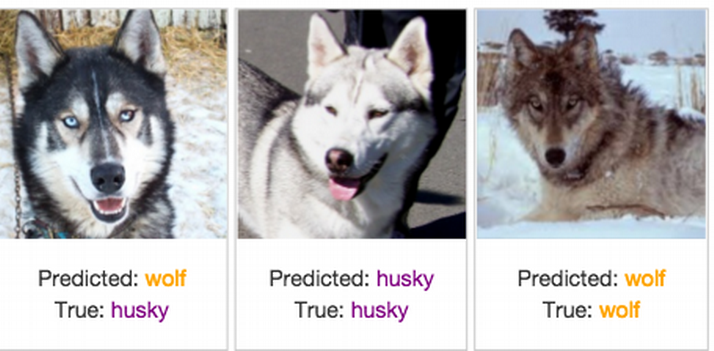
\includegraphics[width=0.58\textwidth]{\pathiml/figure/lime-wolfhusky.png}\\
    		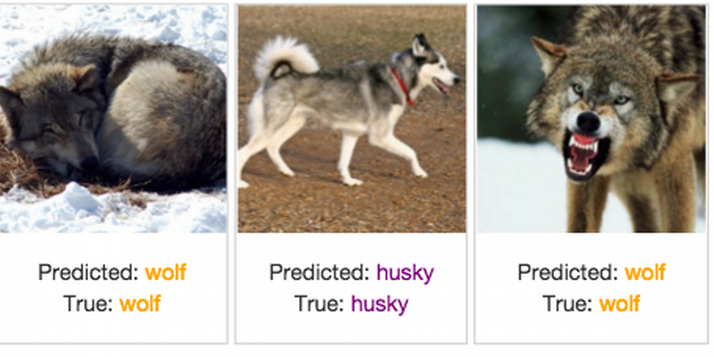
\includegraphics[width=0.58\textwidth]{\pathiml/figure/lime-wolfhusky2.png}
    	\end{center}
	    
	\end{column}
	
	\begin{column}{0.4\textwidth}
	    
	\begin{itemize}
		\item Sometimes the ML model is wrong
		\item Can you guess the pattern the ML model learned to identify a wolf?
	\end{itemize}
	    
	\end{column}
	    
	\end{columns}

\end{frame}


\begin{frame}[c]{Example: Husky or Wolf? Using LIME}

	\begin{columns}
	
	\begin{column}{0.7\textwidth}
	    
	\begin{center}
		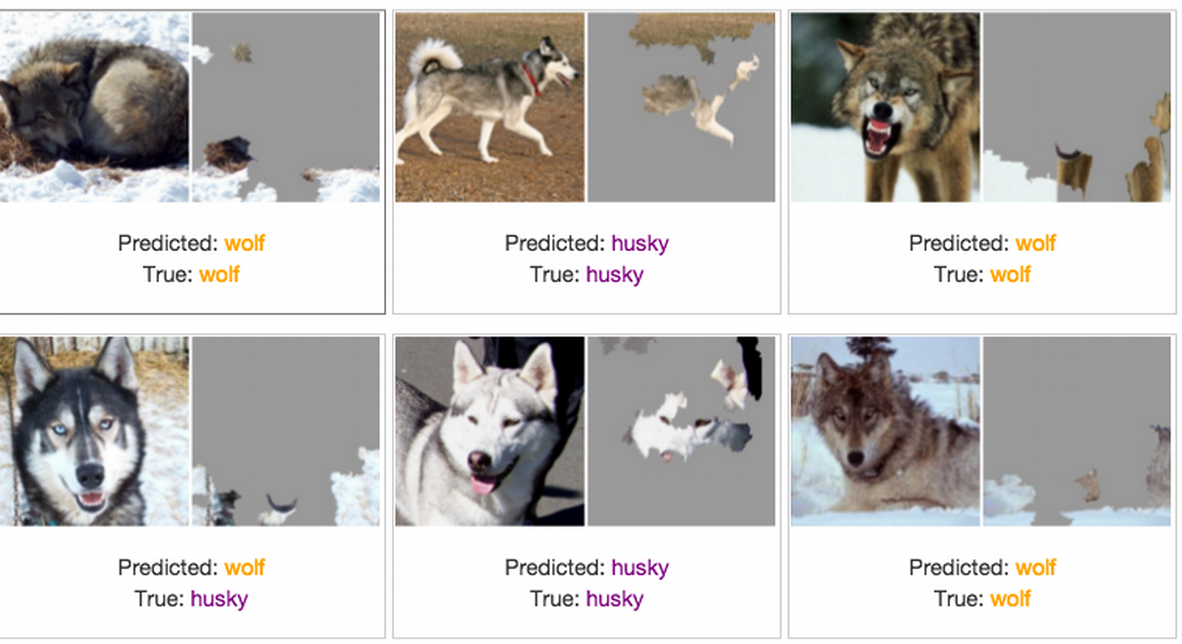
\includegraphics[width=0.9\textwidth]{\pathiml/figure/lime-wolfhusky3.png}
	\end{center}
	    
	\end{column}
	
	\begin{column}{0.3\textwidth}
	    
	\begin{itemize}
		\item Local explanations highlight the parts of an image which led to the prediction
		\item[$\leadsto$] our predictor is actually a snow detector 
	\end{itemize}
	    
	\end{column}
	    
	\end{columns}







\end{frame}


\begin{frame}{Example: Loan Application \citebutton{https://www.elte.hu}{https://www.elte.hu/content/trendfordulo-az-mi-fejlesztesekben.t.19025}}

\begin{columns}[c]
    
    \begin{column}{0.45\textwidth}
        	\begin{center}
		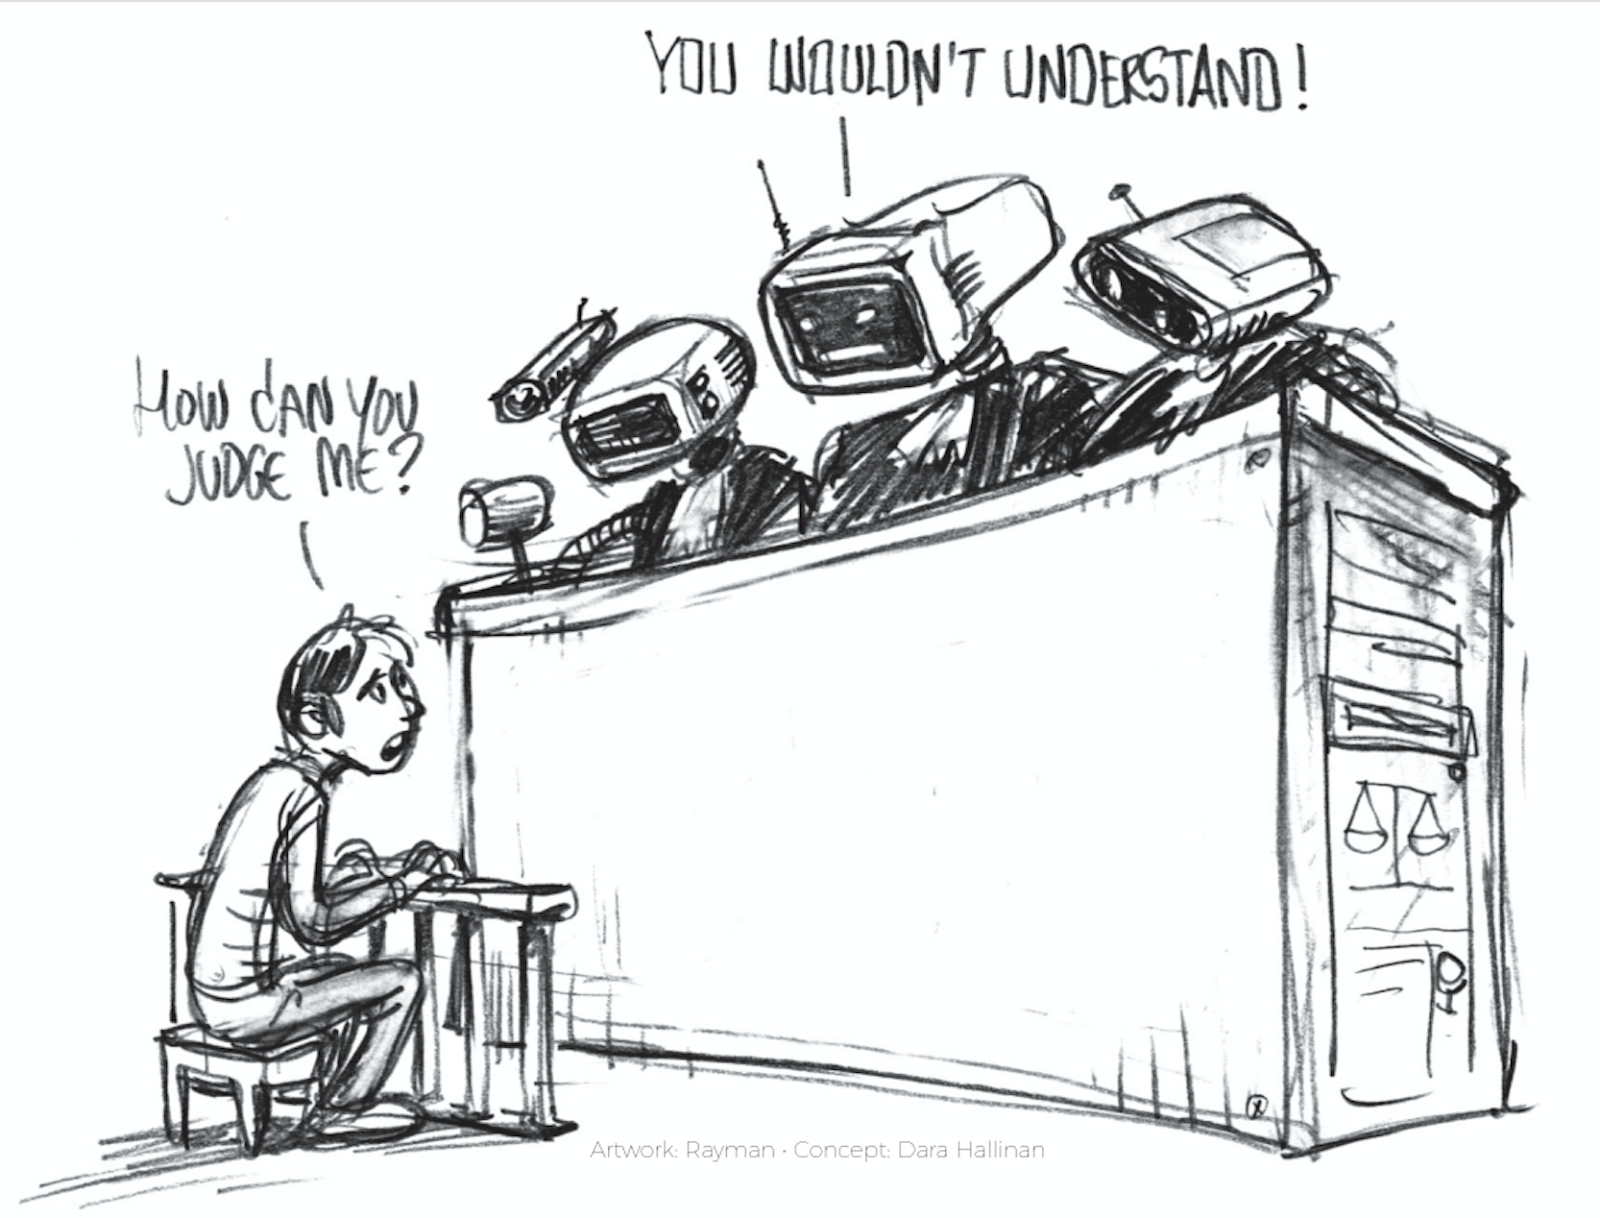
\includegraphics[width=1\textwidth]{\pathiml/figure/IntroJudge.png}
	\end{center}
	
	\end{column}
	
	\begin{column}{0.55\textwidth}
	
    	\begin{itemize}
    	    \item<1-> Imagine: You apply for a loan at an online bank and are immediately rejected without reasons
    	    %Imagine: You are applying at a bank's online portal for a loan and your application gets immediately rejected without reasons
    	    \item<2-> Bank could e.g. provide a counterfactual explanation using local explanation methods:
    	    \begin{itemize}
    	        \item[] ``If you were older than 21, your loan application would have been accepted."
    	    \end{itemize}
    	    \item<3->[$\leadsto$] helps to understand the decision and to take actions for recourse (if req.)
    	\end{itemize}
    	
    \end{column}
\end{columns}

\end{frame}

\begin{frame}[c]{Characteristics of Local Explanations}
	\begin{itemize}[<+->]
		\item \textbf{Explanation scope:} Specific prediction, local environment
		\item \textbf{Model classes:} Model-agnostic by definition, model-specific for computational reasons\\
		$\leadsto$ very popular also for deep learning models
		\item \textbf{Audience:} ML modelers and laypersons
		\item \textbf{Data types:} Often agnostic, including tabular, image, text and audio data
		\item \textbf{Methods:} Many, most prominent are counterfactual explanations, shapley values, local interpretable model-agnostic explanations (LIME), adversarial examples, single ICE curve%, anchors
		%\footnote{For Shapley values and ICE curves see other lectures}
		\item \textbf{Special:} Due to audience, strong interactions with social sciences and strong connections to cognitive science and neurosciences due to data types
	\end{itemize}
\end{frame}

\renewcommand{\titlefigure}{\pathiml/figure/lime5}
\renewcommand{\learninggoals}{
	\item Understand motivation for LIME
	\item Develop a mathematical intuition}

\lecturechapter{LIME}
%\lecture{Interpretable Machine Learning}
\mysectionslide

% Prerequisite: le-intro

% ------------------------------------------------------------------------------
\begin{frame}[c]{LIME}
\begin{itemize}
		\item Local Interpretable Model-agnostic Explanations (LIME) assume that even if a ML model is very complex, the local prediction can be described with a simpler model
		\smallskip\pause
		\item  LIME explains \textbf{individual} predictions of \textbf{any} black-box model by approximating the model \textbf{locally} with an interpretable model
		\smallskip\pause
		\item Called local surrogate models $\leadsto$ often inherently interpretable models such as linear models or classification/regression trees are chosen\\
		\smallskip\pause
		\item LIME should answer why a ML model predicted $\hat y$ for input $\xv$
		\smallskip\pause
		\item LIME is model-agnostic and can handle tabular, image and text data 
\end{itemize}
\end{frame}


\begin{frame}[c]{LIME: Characteristics}

    \textbf{Definition:}\\
	LIME provides a local explanation for a black-box model $\fh$ in form of a model $\gh \in \Gspace$ with $\Gspace$ as the class of potential (interpretable) models\\[2em]
	
	
	Model $g$ should have two characteristics:
	\begin{enumerate}
		\item \textbf{Interpretable}: relation between the input variables and the response are easy to understand  
		\item \textbf{Locally faithful / Fidelity}: similar behavior as $\fh$ in the vicinity of the obs. being predicted
	\end{enumerate}
	
	\vspace{2em}
	Formally, we want to receive a model $\gh$ with \textbf{minimal complexity and maximal local-fidelity} 
\end{frame}


\begin{frame}{Model Complexity}
    
    We can measure the complexity of a model $\gh$ using a complexity measure $J(\gh)$ \lz

 	\textbf{Example: Linear model}\\
 	\begin{itemize}
 	    \item Let $\Gspace = \left\{g: \Xspace \to \R ~|~g(\xv) = s(\thetab^\top \xv)\right\}$ be the class of generalized linear models
 	    \item $s(\cdot)$: identity function for linear regression or logistic sigmoid function for logistic regression
 	    \item[$\leadsto$] $J(g) = \sum_{j = 1}^p \Ind_{\{ \theta_j \neq 0 \}}$ could be the L$_0$ loss, i.e., the number of non-zero coefficients 
 	\end{itemize}
 	\lz\pause
 	
 	\textbf{Example: Tree}\\
 	\begin{itemize}
 	    \item Let $\Gspace = \left\{g:\Xspace \to \R ~|~g(\xv) = \sum_{m=1}^M c_m \Ind_{\{ \xv \in Q_m \}}\right\}$ be the class of trees\\
 	     i.e., the class of additive models (e.g., constant $c_m$)  over the leaf-rectangles $Q_m$
 	    \item[$\leadsto$] $J(g)$ could measure the number of terminal/leaf nodes
 	\end{itemize}
 	
\end{frame}
 
\begin{frame}{Local model fidelity}
 	\begin{itemize}
 		\item $g$ is locally faithful to $\fh$ w.r.t. $\xv$ 
 		if for $\zv \in \Zspace \subseteq \R^p$ close to $\xv$, predictions of $\gh(\zv)$ are close to $\fh(\zv)$ 
 		\item In an optimization task: the closer $\zv$ is to $\xv$, the closer $\gh(\zv)$ should be to $\fh(\zv)$  
 		\pause
 		\item Two required measures:
 		\begin{enumerate}
 			\item A proximity (similarity) measure $\neigh(\zv)$ between $\zv$ and $\xv$, e.g. the exponential kernel:
 			$$\neigh(\zv) = exp(-d(\xv, \zv)^2/\sigma^2)$$ 
 			with $\sigma$ as the kernel width and $d$ as the Euclidean distance (numeric features) or the Gower distance (mixed features) 
 			\pause
 			\item A distance measure or loss function $L(\fh(\zv), \gh(\zv))$, e.g. the L$_2$ loss/squared error
 			$$L(\fh(\zv), \gh(\zv)) = (\gh(\zv) - \fh(\zv))^2$$ 
 		\end{enumerate}
 		\pause
 		\item Given points $\zv$, we can measure local fidelity of $g$ with respect to $\fh$ in terms of a weighted loss
 		$$ L(\fh, g, \neigh) = \sum_{\zv \in \Zspace} \neigh(\zv) L(\fh(\zv), \gh(\zv)) $$
 		%\item Note that identifying \textbf{locally} faithful explanations that are interpretable is less of a challenge than identifying \textbf{globally} faithful explanations. Yet, global fidelity implies local fidelity but not vice versa.
 	\end{itemize}
\end{frame}

\begin{frame}[c]{Minimization task}
	\begin{itemize}
		\item Optimization objective of LIME: 
		$$ \argmin_{g \in \Gspace} L(\fh, \gh, \neigh) + J(g)$$
		\item In practice:
		\begin{itemize}
		    \item LIME only optimizes $L(\fh, \gh, \neigh)$ (model-fidelity) 	
		    \item Users decide threshold on model complexity $J(g)$ beforehand
		\end{itemize}
		\item Goal: \textbf{model-agnostic} explainer
		\begin{itemize}
    		\item[$\leadsto$] optimize $L(\fh, \gh, \neigh)$ without making any assumptions about $\fh$ 
    		\item[$\leadsto$] learn $\gh$ only approximately  
		\end{itemize}
		\end{itemize}
\end{frame} 

\begin{frame}[c]{LIME Algorithm: Outline}
		
		\textbf{Input}:
		\begin{itemize}
		    \item Pre-trained model $\fh$
		    \item Observation $\xv$ whose prediction $\fh(\xv)$ we want to explain
		    \item Model class $\Gspace$ for local surrogate (to limit the complexity of the explanation)
		\end{itemize}
		
		\pause
		\medskip
		
		\textbf{Algorithm}:
		\begin{enumerate}
    		\item Independently sample new points $\zv \in \Zspace$ 
    		\item Retrieve predictions $\fh(\zv)$ for obtained points $\zv$ 
    		\item Weight $\zv \in \Zspace$ by their proximity $\neigh(\zv)$
    		\item Train an interpretable surrogate model $g$ on weighted data points $\zv \in \Zspace$\\ $\leadsto$ predictions $\fh(\zv)$ are the target of this model
    		\item Return the interpretable model $\gh$ as the explainer
		\end{enumerate}
		

	
\end{frame} 

\begin{frame}[c]{LIME Algorithm: Example}

    	\textbf{Illustration} of LIME based on a classification task:
		\begin{itemize}
			\item Light/dark gray background: prediction surface of a classifier
			\item Yellow point: $\xv$ to be explained
			\item $\Gspace$: class of logistic regression models 
		\end{itemize}
		\begin{center}
			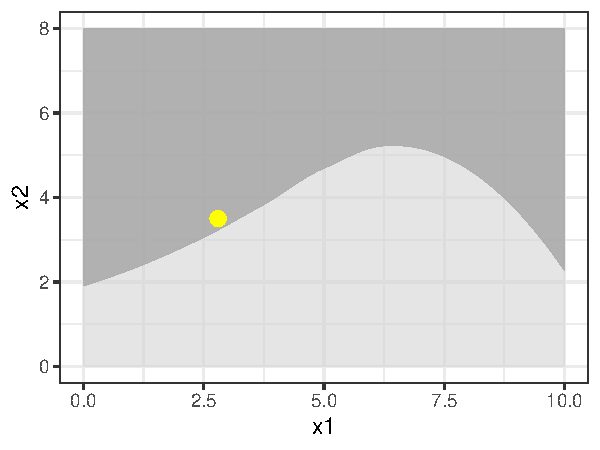
\includegraphics[width=0.35\textwidth]{\pathiml/figure/lime2}
		\end{center}

\end{frame} 


\begin{frame}[c]{LIME Algorithm: Example (Step 1+2: Sampling) \citebutton{Ribeiro. 2016}{https://github.com/marcotcr/lime}}
		
		Strategies for sampling: 
		\begin{itemize} 
			\item Uniformly sample new points from the feasible feature range 
			\item Use the training data set with or without perturbations
			\item Draw samples from the estimated univariate distribution of each feature
			\item Create an equidistant grid over the supported feature range  
		\end{itemize}
		\vspace{-.5cm}
		\begin{columns}
        \begin{column}{0.5\textwidth}  %%<--- here
            \begin{figure}
             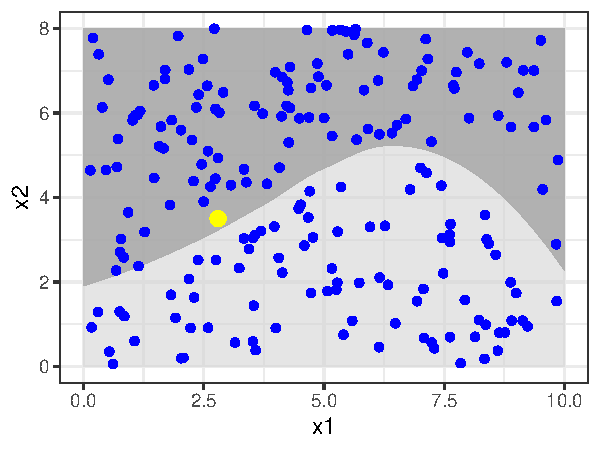
\includegraphics[width=.8\textwidth]{\pathiml/figure/lime3} 
             \vspace{-0.3cm}
             \caption{Uniformly sampled}
             \end{figure}
        \end{column}
        \begin{column}{0.5\textwidth}  %%<--- here
		    \begin{figure}
			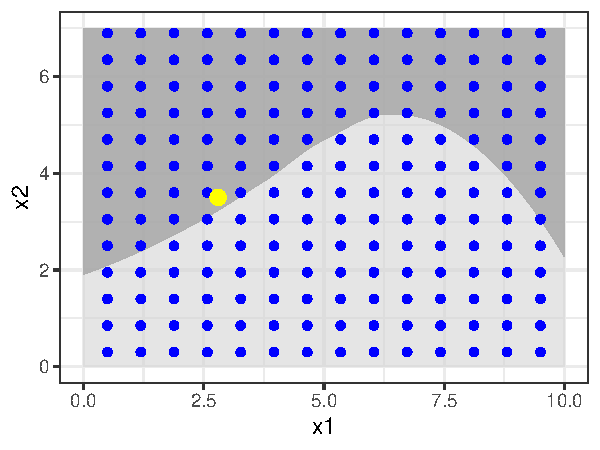
\includegraphics[width=.8\textwidth]{\pathiml/figure/lime3a}
			  \vspace{-0.3cm}
    		    \caption{Equidistant grid}
    		\end{figure}   
    \end{column}
\end{columns}
\end{frame}
		
\begin{frame}{LIME Algorithm: Example (Step 3: Proximity) \citebutton{Ribeiro. 2016}{https://github.com/marcotcr/lime}}

	In this example, we use the exponential kernel defined on the Euclidean distance $d$
		 $$\neigh(\zv) = exp(-d(\xv, \zv)^2/\sigma^2).$$ 
		\begin{center}
			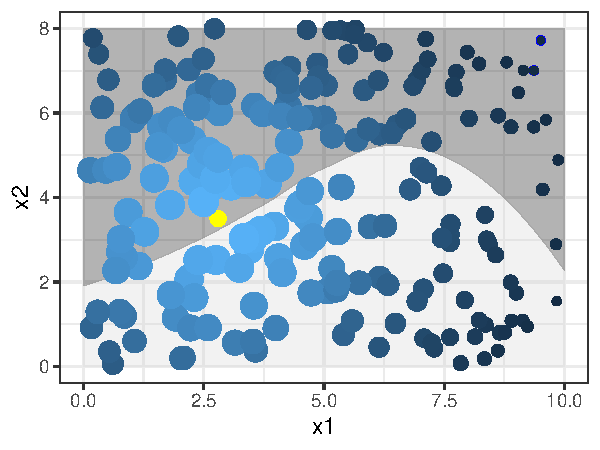
\includegraphics[width=0.4\textwidth]{\pathiml/figure/lime4}
		\end{center}
		
% MARIUS: Not relevant for the example; if we want to introduce it, we should do it somewhere else
% 	An alternative is the Gower proximity: 
% 	$\neigh(\zv) = 1 - \Gower(\zv, \xv) =  1 - \frac{1}{p}\sum_{j = 1}^{p} \delta_G(z_j, x_j) $ 
% 	$\textnormal{ with } \delta_G(z_j, x_j) = 
% 	\begin{cases}
% 	\frac{1}{\widehat{R}_j}|z_j- x_j| & \text{if $x_j$ and $z_j$ are numerical} \\
% 	\mathbb{I}_{z_j \neq x_j} & \text{if $x_j$ and $z_j$ are categorical}
% 	\end{cases}.$
		
\end{frame}
		
\begin{frame}[c]{LIME Algorithm: Example (Step 4: Surrogate) \citebutton{Ribeiro. 2016}{https://github.com/marcotcr/lime}}
		In our example, we fit a \textbf{logistic regression} model (consequently, $L(\fh(\zv), \gh(\zv))$ is the Bernoulli loss)
		\begin{center}
			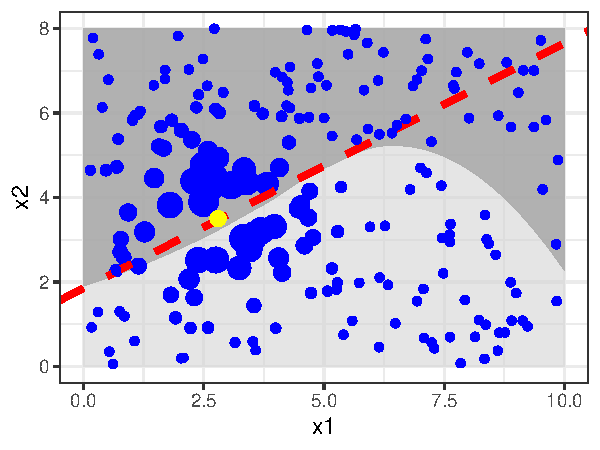
\includegraphics[width=0.4\textwidth]{\pathiml/figure/lime5}
		\end{center}
\end{frame}

%\endlecture

\renewcommand{\titlefigure}{\pathiml/figure/lime_credit_ice2.pdf}
\renewcommand{\learninggoals}{
    \item See real-world data examples
    \item See application to image and text data}

\lecturechapter{LIME Examples}
%\lecture{Interpretable Machine Learning}
\mysectionslide

% Prerequisite: le-intro

% ------------------------------------------------------------------------------

\begin{frame}[c]{Example on Credit Dataset (Tabular)}
	\begin{itemize}
		\item Model: SVM with RBF kernel
		\item $\xv$: first data point of the dataset with $\fh_{bad}(\xv) = 0.658$
		\item $\zv$: training data $\leadsto$ weighted by the Gower proximity 
		\item Surrogate model $\gh$: L$_1$-regularized linear model with 5 features 
	\end{itemize}

    \bigskip

	\begin{table}[ht]
		\centering
		\scriptsize
		\begin{tabular}{rlrlllrrl}
			\hline
			age & sex & job & housing & saving & checking & credit.amount & duration & purpose \\ 
			\hline
			 22 & female &   2 & own & little & moderate & 5951 &  48 & radio/TV \\ 
			\hline
		\end{tabular}
	\end{table}

\end{frame}

\begin{frame}[c]{Example on Credit Dataset (cont'd)}


\begin{center}
	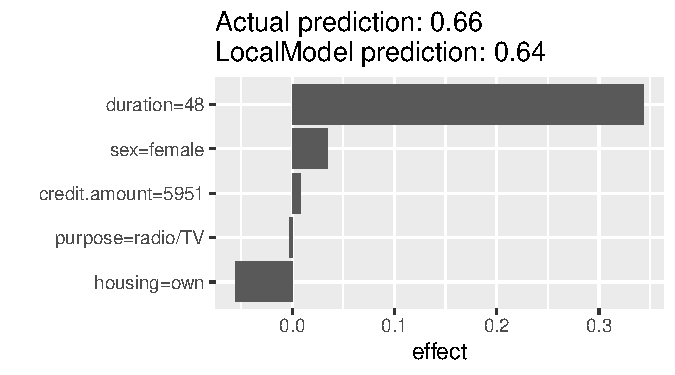
\includegraphics[width=0.45\textwidth]{\pathiml/figure/lime_credit.pdf}\\
	{Effects of surrogate model, i.e. $\thetah^T \xv$}
\end{center}

\begin{itemize}
	\item The local model prediction for $\xv$ is $\gh(\xv) = 0.64$ vs. $\fh(\xv) = 0.658$ 
	\item $\gh$ has a local fidelity of $L(\pih, \gh, \neigh) = 4.82$ with $\neigh(\zv)$ as the Gower proximity and $L(\pih_{bad}(\zv), g(\zv))$ as the euclidean distance 
\end{itemize}

\end{frame}
	
\begin{frame}[c]{Example on Credit Dataset (cont'd)}

\begin{itemize}	
	\item 2-dim ICE plots (aka. prediction surface plot) of credit amount and duration show how the surrogate model $g$ linearly approximates the previously nonlinear prediction surface of $\pih_{bad}$ 
\end{itemize}
\vspace{-0.4cm}
 \begin{columns}
	\begin{column}{0.47\textwidth}
		\begin{center}
		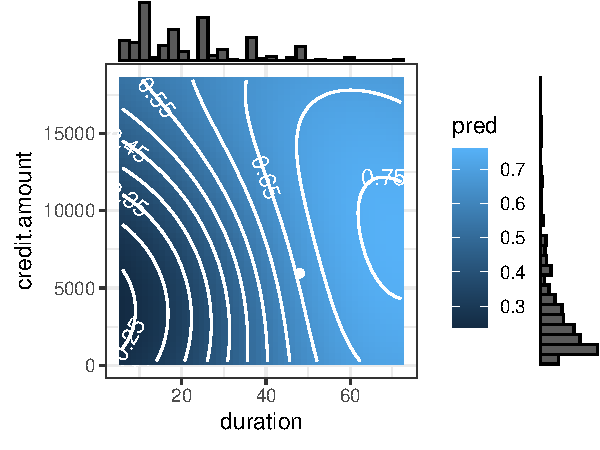
\includegraphics[width=1\textwidth]{\pathiml/figure/lime_credit_ice1.pdf}
		\end{center}		
	\end{column}
	\begin{column}{0.46\textwidth}  
		\begin{center}
				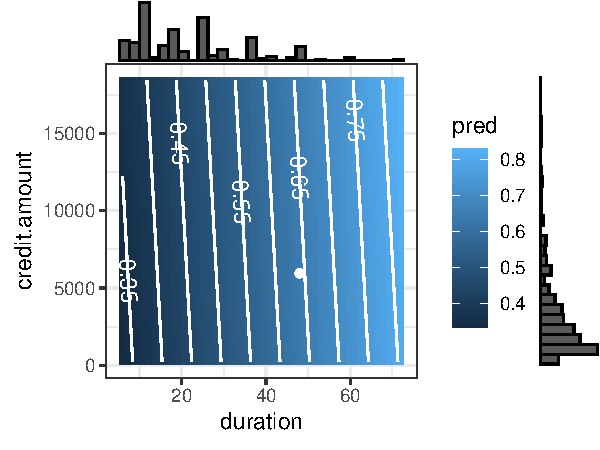
\includegraphics[width=1\textwidth]{\pathiml/figure/lime_credit_ice2.pdf}
		\end{center}
			
	\end{column}
\end{columns}
\vspace{-0.4cm}
\begin{center}
		{2-dim ICE plot of $\fh_{bad}$ (\textbf{left}) and surrogate $g$ (\textbf{right}) for features duration and credit amount. \\The white dot is $\xv$. The histograms display the marginal distribution of the training data $\Xmat$.}
\end{center}

\end{frame}

%\begin{frame}[containsverbatim,allowframebreaks]{Bike Sharing Dataset}
%\vspace{-.3cm}
%
%\begin{center}
%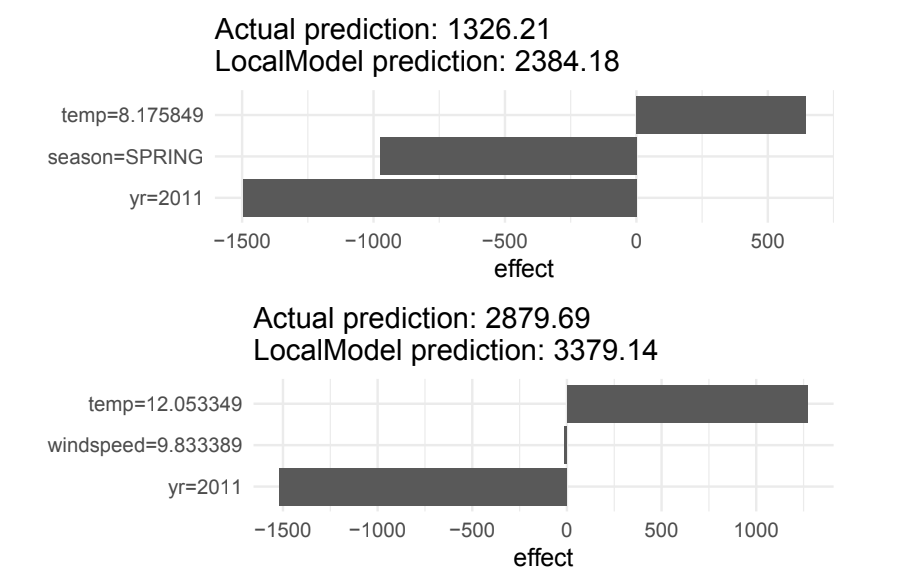
\includegraphics[width=0.7\textwidth]{\pathiml/figure/bike-figure.png}
%\end{center} 
%
%\footnotesize \textbf{Figure:} LIME for two example instances of the bike sharing dataset.
%
%\normalsize
%\vspace{0.2cm}
%The plots show the feature effect of the sparse linear model, i.e. the model coefficients times the feature value of the instance.
%Warmer temperature has a positive effect on the prediction, 
%while the year 2011 has a large negative effect as well as the springtime.
%\end{frame}

\begin{frame}{LIME for Text Data \citebutton{Shen, Ian, (2019)}{https://medium.com/just-another-data-scientist/explain-sentiment-prediction-with-lime-f90ae83da2da}}
    LIME can also be applied to text data: 
	\begin{itemize}
		\item Raw text representations: 
		\begin{itemize}
		    \item Binary vector indicating the presence or absence of a word 
		    \item A vector of word counts
		\end{itemize}
		\item Examples for \textit{``This text is the first text."} and \textit{``Finally, this is the last one."}:
		\begin{center}
			\begin{tabular}{c|c|c|c|c|c|c|c} 
				this & text & is & the & first & finally & last & one \\ 
				\hline
				1 & 2 & 1 & 1 & 1 & 0 & 0 & 0 \\
				1 & 0 & 1 & 1 & 0 & 1 & 1 & 1 \\
			\end{tabular}
		\end{center} 
		\item \textbf{Sampling}: Randomly set the entry of individual words to $0$; equal to removing all occurrences of this word in the text. 
		\item \textbf{Proximity}: Exponential kernel with cosine distance. 
		\begin{itemize}
		    \item Neglects words that do not occur in both texts 
		    \item Measures the distance irrespective of the text size
		\end{itemize}
	\end{itemize}
\end{frame}
	
\begin{frame}{LIME for Text Data (cont'd) \citebutton{Shen, Ian, (2019)}{https://medium.com/just-another-data-scientist/explain-sentiment-prediction-with-lime-f90ae83da2da}}	 
	\begin{itemize}
		\item Random forest classifier labeling movie reviews from IMDB 
		\begin{itemize}
		    \item \textcolor{blue}{0}: negative
		    \item \textcolor{orange}{1}: positive
		\end{itemize}
		\item Surrogate model is a sparse linear model 
	\end{itemize}
	
	\begin{figure}
		\begin{center}
			%\captionsetup{font = scriptsize, labelfont = {bf, scriptsize}}
			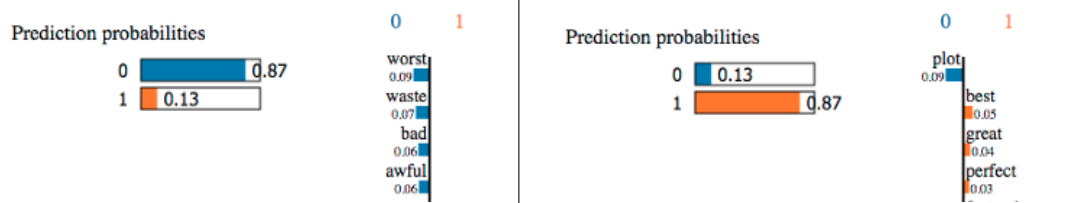
\includegraphics[width=0.9\textwidth]{\pathiml/figure/lime_movier}
		\end{center}
	\end{figure}
	
	{Words like ``worst`` or ``waste`` indicate negative review while words like ``best`` or ``great`` indicate positive review}
	
	\end{frame}
	
\begin{frame}[c]{LIME for image data}
	\begin{columns}
		\begin{column}{0.67\textwidth}
			LIME also works for image data:  
			\begin{itemize}
				\item \textbf{Idea}: Each obs. is represented by a binary vector indicating the presence or absence of superpixels \citebutton{Achanta et al. 2012}{https://ieeexplore.ieee.org/document/6205760}
				\item Superpixels are interconnected pixels with similar colors (absence of a single pixel might not have a (strong) effect on the prediction)
				\item \textbf{Warning}: Size of superpixels needs to be determined before the segmentation takes place
				\item \textbf{Sampling}: Randomly switching some of the super pixels ``off", i.e., by coloring some superpixels uniformly
			\end{itemize}		
		\end{column}
		\begin{column}{0.26\textwidth}  
			\begin{center}
				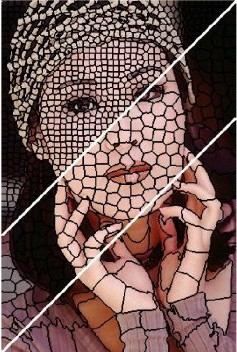
\includegraphics[width=1\textwidth]{\pathiml/figure/superpixel_woman}
				{Example for superpixels of different sizes}
			\end{center}
		\end{column}
	\end{columns}
    
\end{frame}
\begin{frame}{LIME for image data (cont'd) \citebutton{Ribeiro. 2016}{https://github.com/marcotcr/lime}}
	\begin{itemize}
		\item Explaining prediction of pre-trained inception neural network classifier
		\item \textbf{Sampling}: Graying out all superpixels besides 10 superpixels
		\item \textbf{Surrogate}: Locally weighted sparse linear models 
		\item \textbf{Proximity}: Exponential kernel with euclidean distance
	\end{itemize}
% https://lime-ml.readthedocs.io/en/latest/lime.html#module-lime.lime_image
	\vspace{-0.3cm}
	\begin{center}
		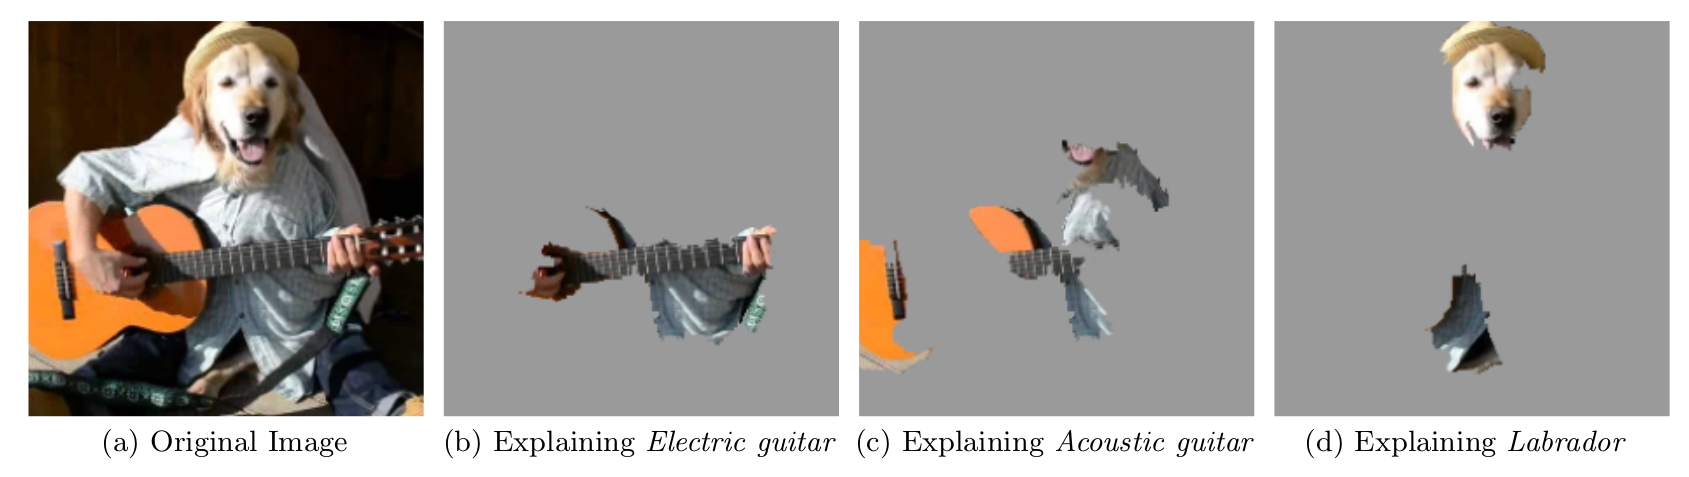
\includegraphics[width=0.8\textwidth]{\pathiml/figure/lime-images}
		
		{Top 3 classes predicted}
	\end{center}
	
\end{frame}
%\endlecture

	\renewcommand{\titlefigure}{\pathiml/figure/lime5}
    \renewcommand{\learninggoals}{
    	\item Learn why LIME should be used with caution
    	\item Possible pitfalls of LIME}
	
	\lecturechapter{LIME Pitfalls}
	%\lecture{Interpretable Machine Learning}
	\mysectionslide
	
	% Prerequisite: le-into, le-lime
	
	% ------------------------------------------------------------------------------


\begin{frame}[c]{LIME Pitfalls}
  \begin{itemize}
  	\item %Despite being a popular interpretation method, several papers caution to be careful in LIME
  	LIME is one of the best known interpretable ML methods\\ 
  	$\leadsto$ But several papers caution to be careful in practice 
  	\item Problems can occur on different levels which are described subsequently: 
  	\begin{itemize}
  	    \item Sampling procedure (extrapolation)
  	    \item Definition of locality (sensitivity)
  	    \item Scope of feature effects (local vs. global)
  	    \item Faithfulness (trade-off with sparsity)
  	    \item Surrogate model (hiding biases, robustness)
  	    \item Definition of superpixels in case of image data (sensitivity)
  	\end{itemize}
  	%\item These are discussed in more detail in the following 
  \end{itemize}
  
\end{frame}
  
\begin{frame}[c]{Pitfall: Sampling}
	\begin{itemize}
	\itemsep1em
	  \item \textbf{Pitfall}: Common sampling strategies for $\zv \in Z$ do not account for correlation between features 
      \item \textbf{Implication}:  Unlikely data points might be used to learn local explanation models
      \pause
      \item \textbf{Solution I}: Conditional sampling\\ %Use a local sampler directly on $\Xspace$\\
      $\leadsto$ particularly difficult for high dimensional or mixed feature spaces 
      \item \textbf{Solution II}: Use training data to fit surrogate model\\
      $\leadsto$ only works well with enough data near $\xv$
    \end{itemize}
    
\end{frame}

\begin{frame}[c]{LIME Pitfall: Locality}

	\begin{itemize} 
     \item \textbf{Pitfall}: Difficult to define locality (= how samples are weighted locally) \\
    % \begin{itemize}
     %    \item[$\leadsto$] 
     $\leadsto$ Strongly affects local model, but there is no automatic procedure for choosing neighborhood
     %\end{itemize}
     \item Originally, an exponential kernel as proximity measure between $\xv$ and $\zv$ was proposed:\\
     	$\neigh(\zv) = exp(-d(\xv, \zv)^2/\sigma^2)$ where $d$ is a distance measure and $\sigma$ is the kernel width 
    %  	 \begin{center}
    %  		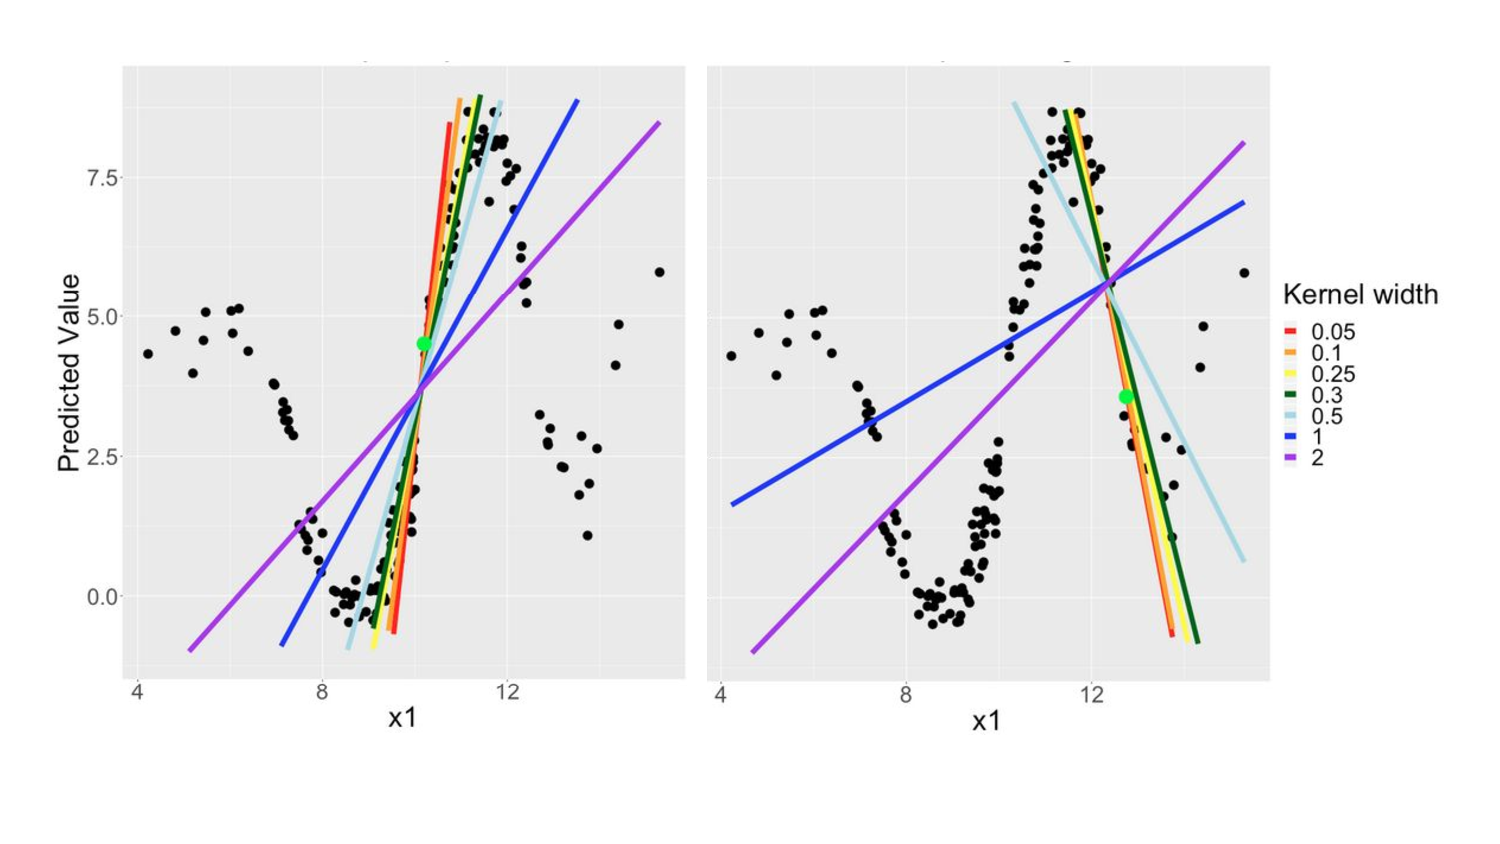
\includegraphics[width=0.6\textwidth]{\pathiml/figure/lime_locality}
    %  		\vspace{-0.5cm}
     		
    %  		\scriptsize{Linear surrogate models for two observations based on the same model with one target and one feature. Each line displays one linear surrogate model with different kernel width. In the right figure, larger kernel sizes are more severe.}
     		
    %  	\end{center}
     \end{itemize}
     \pause
     \begin{columns}[T, totalwidth=\linewidth]
        \begin{column}{0.65\textwidth}
        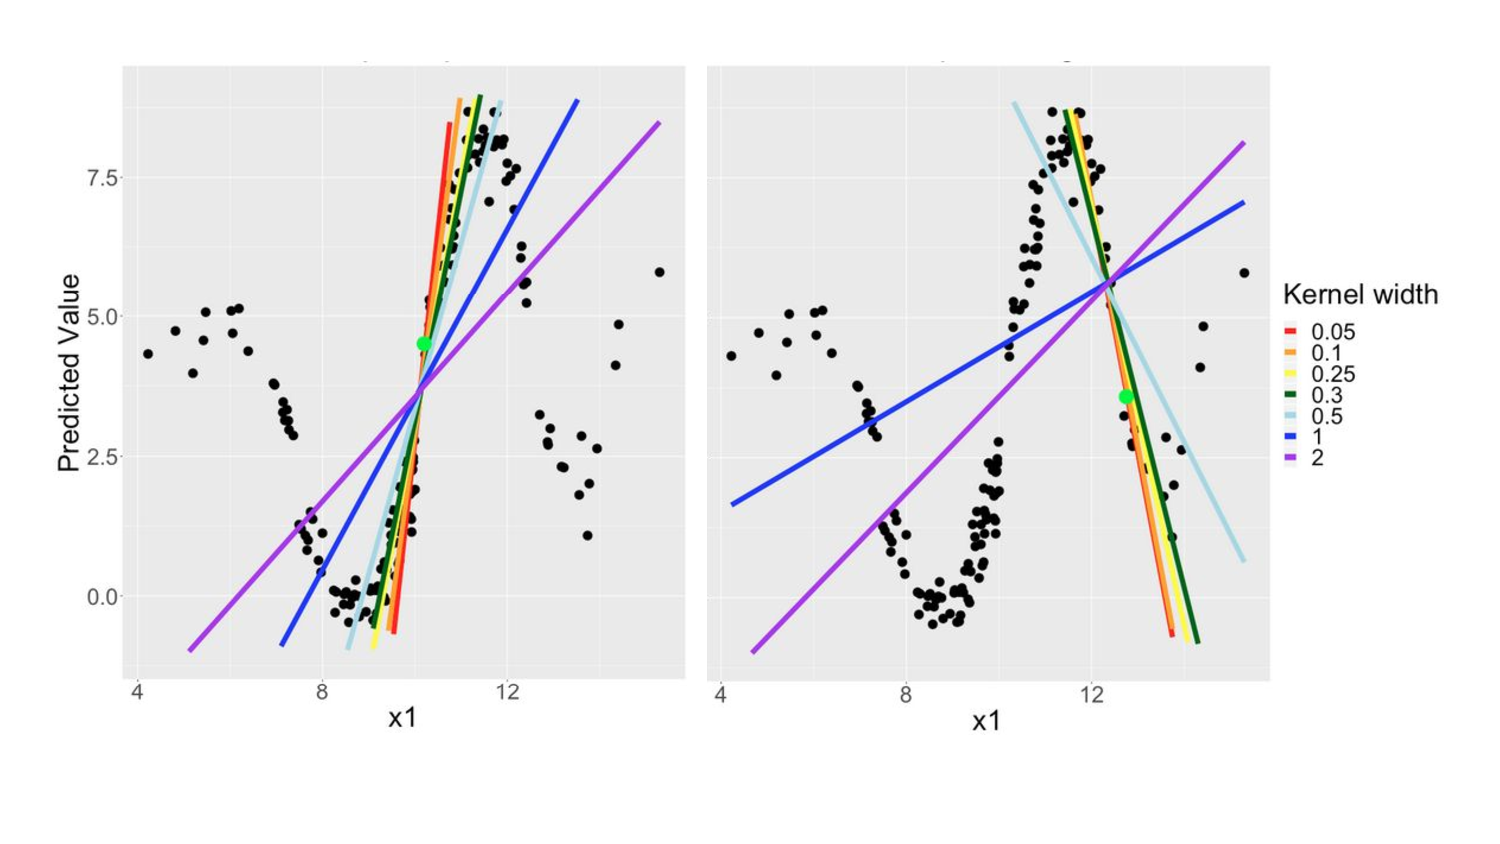
\includegraphics[width=\textwidth, trim = 0px 0px 30px 40px, clip]{\pathiml/figure/lime_locality}
         \end{column}
         \begin{column}{0.35\textwidth}
         \begin{itemize}
             \item Surrogate models for 2 obs. (green points) for same model with one feature $x_1$
             \item Each line refers to a linear surrogate model with different kernel width
             \item Right figure: larger kernel widths influence lines more
         \end{itemize}
         \end{column}
     \end{columns}
\end{frame}

\begin{frame}[c]{LIME Pitfall: Locality \citebutton{Kopper et al. 2019}{https://slds-lmu.github.io/iml_methods_limitations/}}
    \begin{itemize} 
         \item \textbf{Solution I}: Kernel width strongly interacts with locality:
         \begin{itemize}
             \item Large kernel width leads to interaction with points further away (unwanted)
             \item Small kernel width leads to small neighborhood\\
             $\leadsto$ risk of few data points\\
             $\leadsto$ potentially fitting more noise
         \end{itemize}
         \pause
    	\item \textbf{Solution II}: Use Gower distance where no kernel width needs to be specified 
    	\begin{itemize}
    	    \item \textbf{Problem}: data points far away receive weight $ > 0$\\
    	    $\leadsto$ resulting explanations are rather global than local surrogates   
    	\end{itemize}
    \end{itemize}
\vspace{0.3cm}

\end{frame}

\begin{frame}[c]{Pitfall: Local vs. Global Features \citebutton{Laugel et al. 2018}{https://arxiv.org/pdf/1806.07498.pdf}}

\begin{itemize}%[<+->]
	\item<1-> \textbf{Problem}: \\
	By sampling obs. for the surrogate model from the whole input space, the influence of local features might be hidden in favor of features with global influence (even for small kernel width)
	\item<2-> \textbf{Implication}: 
	\begin{itemize}
	    \item Some features influence the \textbf{global} shape of the black-box model
	    \item Other \textbf{local} features impact predictions only in smaller regions of $\Xspace$ %for a small area of $\Xspace$ 
	\end{itemize}
	\item<3-> \textbf{Example}: Decision trees\\
	$\Rightarrow$ Split features close to root have a more global influence than the ones close to leaves
\end{itemize}

\end{frame}


\begin{frame}{Pitfall: Local vs. Global Features -- Example \citebutton{Laugel et al. 2018}{https://arxiv.org/pdf/1806.07498.pdf}}

\begin{columns}
	\begin{column}{0.6\textwidth}
		\begin{itemize}
		\item Binary classification model
		\item Right figure: %Given in figure to the right:
		\begin{itemize}
		    \item Black and grey crosses: training data
		    \item Green dot: Obs. to be explained
		    \item Background color: Classification of random forest
		    \item Dark grey curve: Classifier's decision boundary
		    \item Dotted lines: Local decision boundary
		\end{itemize}
		\item \textbf{Observation:} Decision boundaries of LIME with different kernels (blue and green lines) do not match the direction of the local decision boundary\\ (which appears steeper)
	\end{itemize}
\end{column}
\begin{column}{0.39\textwidth}
%\vspace{0.3cm}

	\begin{center}
	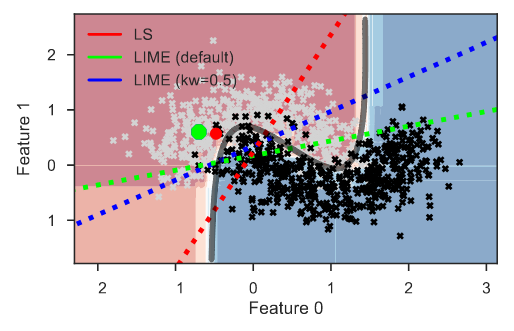
\includegraphics[width=1\textwidth]{\pathiml/figure/lime-globallocal2}

	{Half-moons dataset}
	
\end{center}

	\end{column}
\end{columns}
%\footnote[frame]{Laugel et al. (2018). Defining Locality for Surrogates in Post-hoc Interpretability. \url{https://arxiv.org/pdf/1806.07498.pdf}.}
\end{frame}

\begin{frame}{Pitfall: Local vs. Global Features -- Solution \citebutton{Laugel et al. 2018}{https://arxiv.org/pdf/1806.07498.pdf}}
\begin{columns}[T, totalwidth=\textwidth]
	\begin{column}{0.6\textwidth}
	%\vspace{-.5cm}
		\begin{itemize}
		\item \textbf{Solution}: 
		Find closest point to $\xv$ from other class and sample new points $\zv$ around it for higher local accuracy
		\begin{center}
		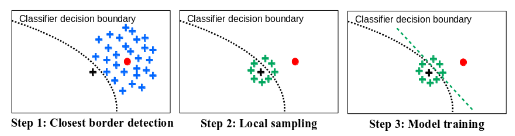
\includegraphics[width=\linewidth]{\pathiml/figure/laugel_method}
		\scriptsize{\textbf{Example:} $\xv$ (red point), closest point from other class (black cross)}
	    %{Local surrogate (LS) method by \citebutton{Laugel et al. 2018}{https://arxiv.org/pdf/1806.07498.pdf}}
		\end{center}
		%Sample new instances $\zv$ around the decision boundary closest from point $\xv$ for higher local accuracy
		\pause
		\item Red dot (right figure): Closest point from other class

		\item Red line: Local surrogate (LS) method \citebutton{Laugel et al. 2018}{https://arxiv.org/pdf/1806.07498.pdf}\\
		$\leadsto$ better approximates the local direction of the decision boundary 
	\end{itemize}
% 	\begin{center}
% 		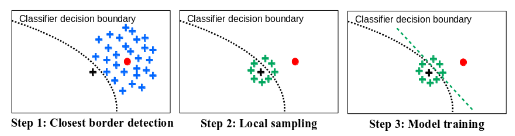
\includegraphics[width=1\textwidth]{\pathiml/figure/laugel_method}
% 	    {Local surrogate (LS) method by \citebutton{Laugel et al. 2018}{https://arxiv.org/pdf/1806.07498.pdf}}
% 		\vspace{-0.3cm}
% 		\end{center}
\end{column}
\begin{column}{0.39\textwidth}
%\vspace{0.3cm}

	\begin{center}
	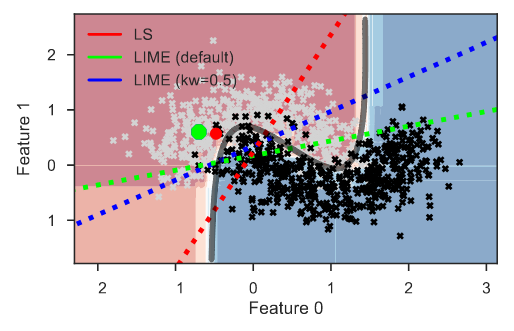
\includegraphics[width=1\textwidth]{\pathiml/figure/lime-globallocal2}
	
	{Half-moons dataset}
	
\end{center}

	\end{column}

\end{columns}
%\footnote[frame]{Laugel et al. (2018). Defining Locality for Surrogates in Post-hoc Interpretability. \url{https://arxiv.org/pdf/1806.07498.pdf}.}
\end{frame}


\begin{frame}[c]{Pitfall: Faithfulness}
\begin{itemize}
%\itemsep1em
	\item \textbf{Problem}: Trade-off between local fidelity vs. sparsity
	\item \textbf{Observation I}: Low fidelity $\leadsto$ unreliable explanations
	\item \textbf{Observation II}: High fidelity requires complex models $\leadsto$ difficult to interpret surrogate model %surrogate model cannot easily be interpreted
	\pause
	\item \textbf{Example: Credit data} 
	\begin{itemize}
	\itemsep0em
	    \item Original prediction by random forest for one data point $\xv$: 
	    $$\fh(\xv) = \hat{\P}(y = 1 ~|~ \xv) = 0.143$$
	    \item %Regularized linear model with only three selected features (\code{sex}, \code{checking.account}, \code{duration}) $g_{lm}(\xv) = 0.283$
	    Linear model with only three selected features (\code{age}, \code{checking.account}, \code{duration}):
	    $$g_{lm}(\xv) = \thetah_0 + \thetah_1 x_{age} + \thetah_2 x_{checking.account} + \thetah_3 x_{duration} = 0.283$$
	    \item Generalized additive model (with all 9 features) is more complex:
    $$%\begin{equation*} 
    %\begin{split}
    g_{gam}(\xv) = \thetah_0 + f_{age}(x_{age}) + f_{checking.account}(x_{checking.account}) + f_{duration}(x_{duration}) +  \dots %& = \thetah_0 + s_{age}(x_{age}) +s_{credit.amount}(x_{credit.amount}) s_{duration}(x_{duration}) + \thetah_{sex = male} \Ind_{sex = male}   \\
    %& + \thetah_{job}(x_{job}) + \thetah_{housing = own} \Ind_{housing = own} +   \thetah_{housing = rent} \Ind_{housing = rent} \\
    %& + \thetah_{saving.accounts = moderate} \Ind_{saving.accounts = moderate} + \thetah_{saving.accounts = rich} \Ind_{saving.accounts = rich} \\
    %& + ... + \thetah_{purpose = radio/TV} \Ind_{purpose = radio/TV}  
    = 0.148$$
    %\end{split}
    %\end{equation*}
	\end{itemize}
\end{itemize}

\end{frame}

\begin{frame}{Pitfall: Hiding biases \citebutton{Slack et al. 2020}{https://arxiv.org/abs/1911.02508}}

\begin{itemize}
	\item \textbf{Problem}: Developer could manipulate their model to hide biases 
	\item \textbf{Observation}: LIME can sample out-of-distribution points (extrapolation)
	\pause
	\item \textbf{Attack} with adversarial model:
	    \begin{enumerate}
	    \item classifier to discriminate between in-distribution and out-of-distribution data points
	    \item for in-distribution points, use the original (biased) model
	    \item for out-of-distribution points produced for local explanation, use an unbiased model
	    \item[$\leadsto$] LIME samples out-of-distribution points and uses the unbiased model for local explanation\\
	    \item[$\leadsto$] this hides the bias of the true model
	    \end{enumerate}
\end{itemize}
	\begin{columns}[T, totalwidth=\linewidth]
		\begin{column}{0.5\textwidth}
	    \centering
	    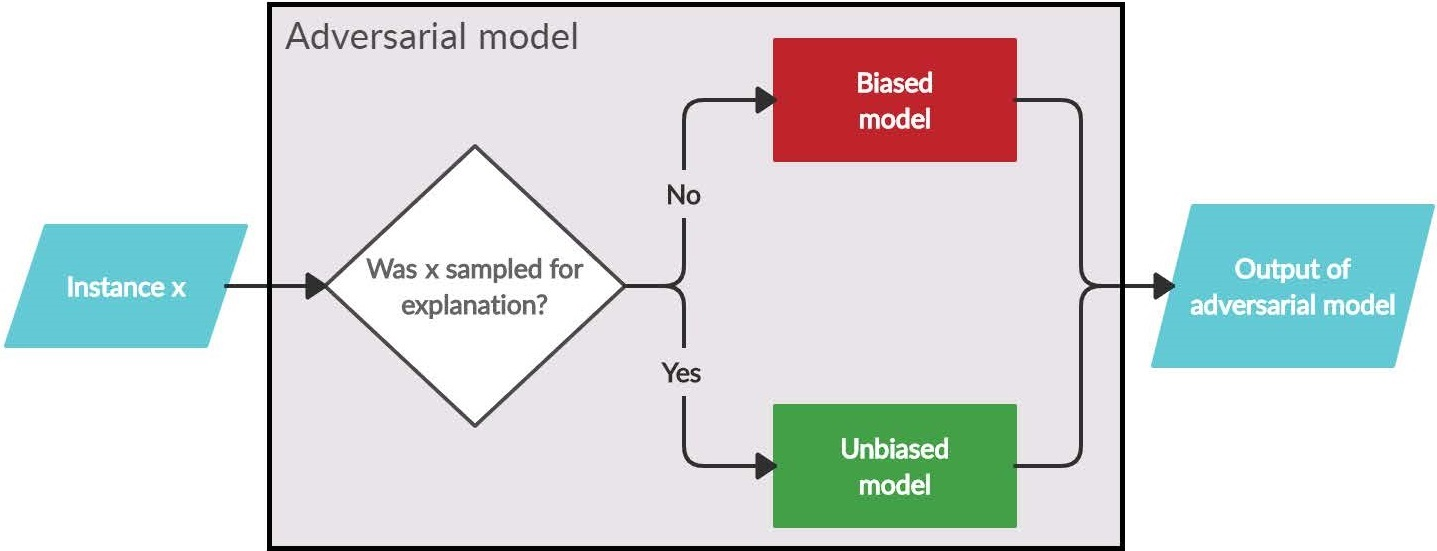
\includegraphics[width=\textwidth]{\pathiml/figure/attack_biased_unbiased.jpg}
	    \citebutton{Vres, Sikonja (2021)}{https://arxiv.org/abs/2101.11702}
	    \end{column}
\pause
	    \begin{column}{0.5\textwidth}
	    \textbf{Example}: Not using `gender` to approve a loan % Credit dataset %
	    \begin{itemize}
	        \item biased model trained on features correlated with `gender` (e.g. duration of parental leave)\\
	        $\leadsto$ used 
	        %for in-distribution points (realistic values) 
	        to make biased / unfair predictions
	        \item unbiased model trained on features uncorrelated with `gender`\\
	        $\leadsto$ used to produce explanations based on unbiased predictions to hide bias
	        %$\leadsto$ used for (extrapolated) LIME samples\\
	        %$\Rightarrow$ produced local explanations seem fair as they are based on unbiased model
	        %could be trained on features uncorrelated with `gender`
	    \end{itemize}
	    \end{column}
	\end{columns}
\end{frame}

\begin{frame}[c]{Pitfall: Robustness \citebutton{Alvarez-Melis, D., \& Jaakkola, T. 2018}{https://arxiv.org/abs/1806.08049}}
\begin{itemize}
	\item \textbf{Problem}: Instability of explanations 
	\item \textbf{Observation}: Explanations of two very close points could vary greatly 
	\begin{itemize}
	    \item[$\leadsto$] can happen because of other sampled data points $\zv$
	\end{itemize}
\end{itemize}
\vspace{-0.7cm}
\begin{columns}
	\begin{column}{0.48\textwidth}
		\begin{center}
		
		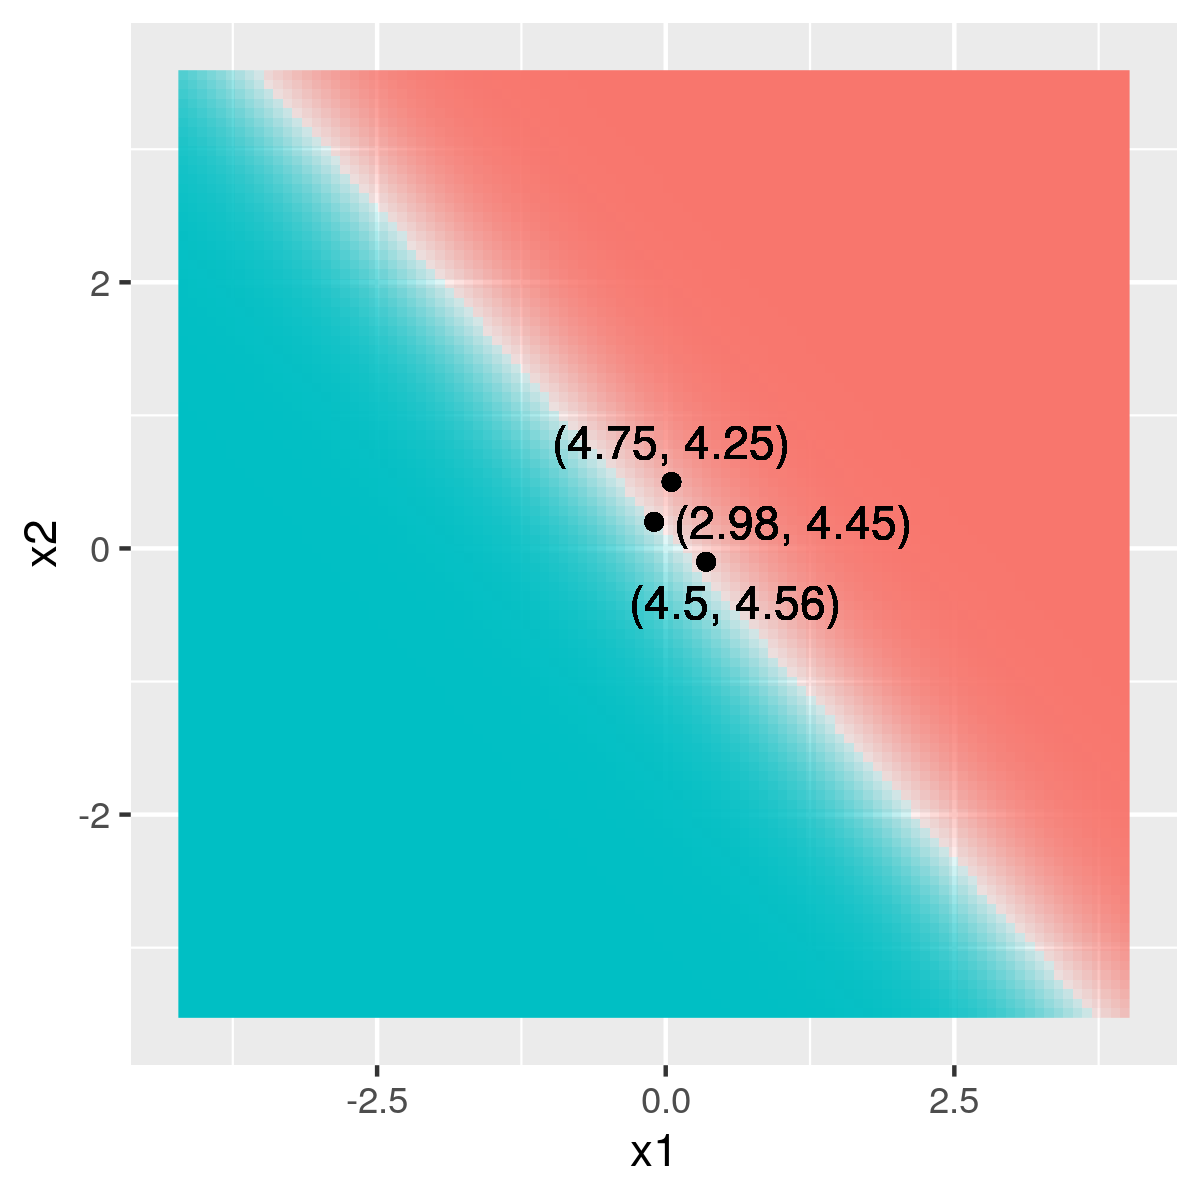
\includegraphics[width=0.55\textwidth]{\pathiml/figure/lime_robustness_1.png}
		
		{Linear prediction task (logistic regression). \\Linear surrogate returns similar coefficients for similar points.}
		
		\end{center}
	\end{column}
	\begin{column}{0.48\textwidth}
		\begin{center}
	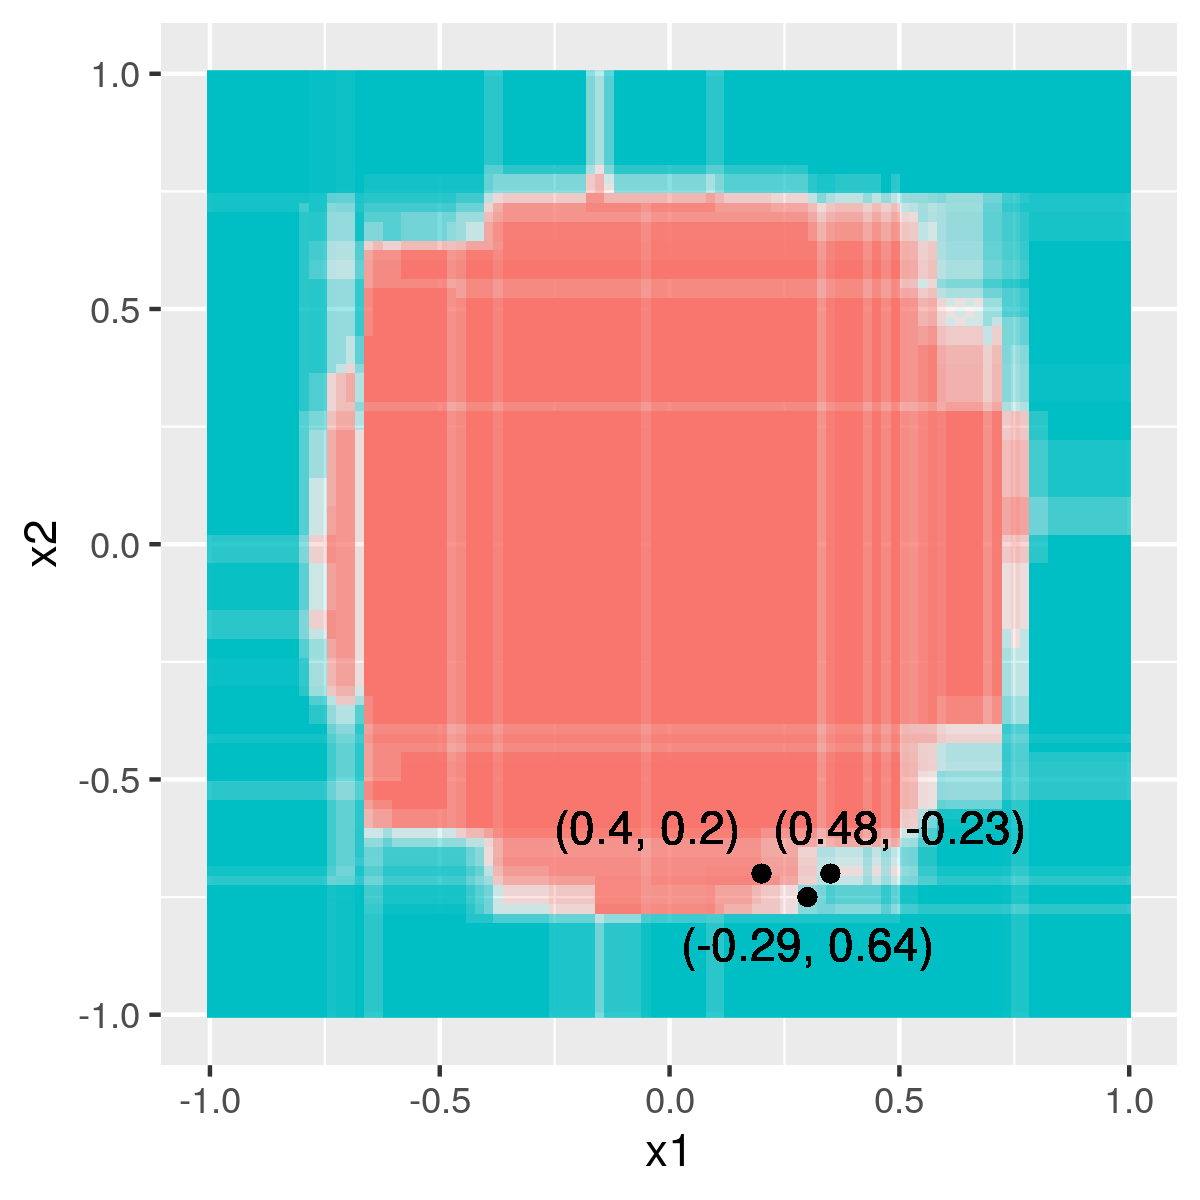
\includegraphics[width=0.55\textwidth]{\pathiml/figure/lime_robustness_2.png}
	
	{Circular prediction task (random forest). \\Linear surrogate returns different coefficients for similar points.}
	
	\end{center}
\end{column}
\end{columns}
\end{frame}

\begin{frame}{Pitfall: Definition of Superpixels \citebutton{Achanta et al. 2012}{https://ieeexplore.ieee.org/document/6205760}}

\begin{columns}
    
    \begin{column}{0.6\textwidth}
        
        \begin{itemize}
        	\item \textbf{Problem}: Instability because of specification of superpixels for image data 
        	\item \textbf{Observation}: Multiple specification of superpixels exist, influencing both the shape and size 
        	\pause
        	\item \textbf{Implication}: The specification of superpixel has a large influence on the explanations 
        	\item \textbf{Attack}: Change superpixels as part of an adversarial attack $\leadsto$ changed explanation
        \end{itemize}
        
    \end{column}
    
    \begin{column}{0.4\textwidth}
    
        \centering
        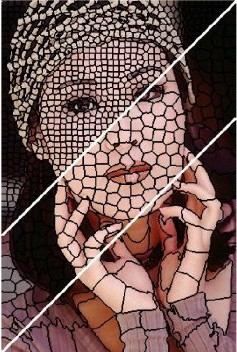
\includegraphics[width=0.7\textwidth]{\pathiml/figure/superpixel_woman}
        
    \end{column}
    
\end{columns}

\end{frame}


%\endlecture

\renewcommand{\titlefigure}{\pathiml/figure/counterfactuals_obj}
\renewcommand{\learninggoals}{
\item Understand the motivation behind CEs
\item See the mathematical foundation of CEs}

\lecturechapter{Counterfactual Explanations}
%\lecture{Interpretable Machine Learning}
\mysectionslide

% ------------------------------------------------------------------------------

\begin{frame}[c]{Example: Credit Risk Application}
	\begin{itemize}
		\item $\textbf{x}$: customer and credit information
		\item $y$: grant or reject credit
	\end{itemize}
	\begin{center}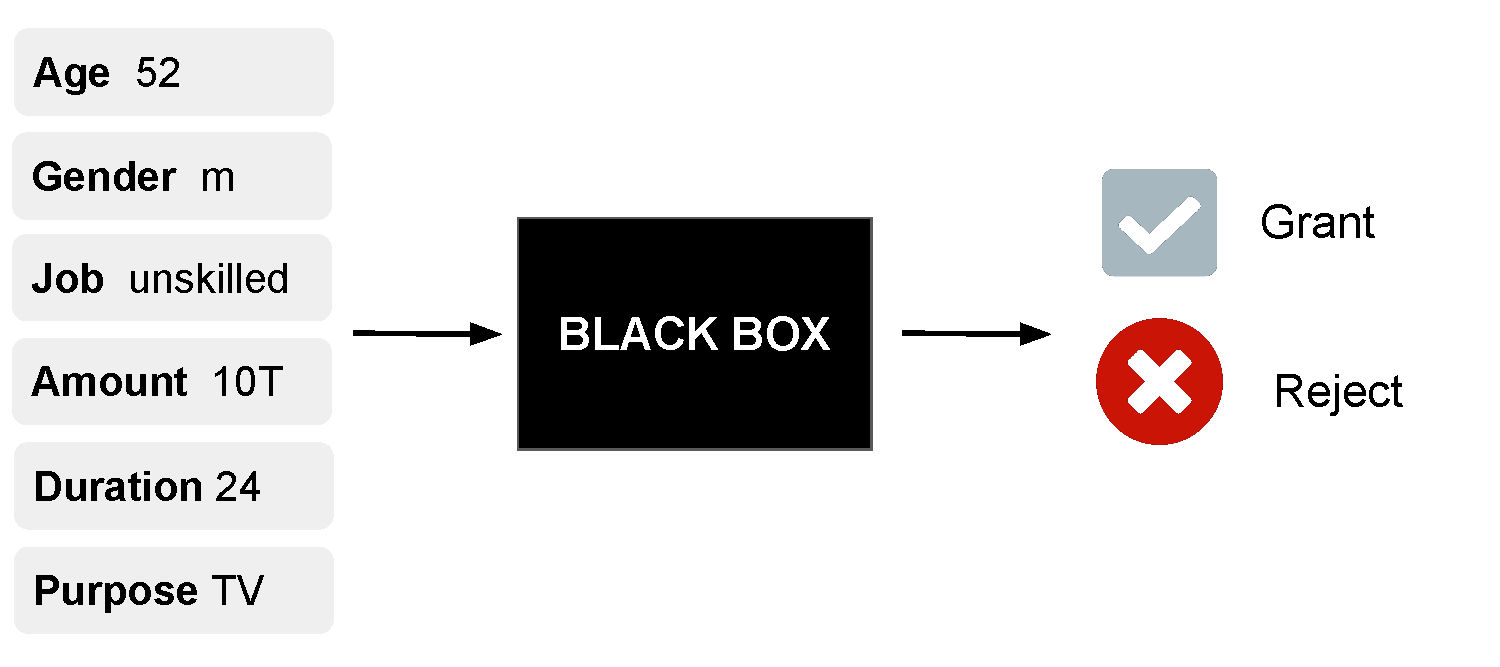
\includegraphics[width=0.6\linewidth, page=1]{\pathiml/figure/counterfactuals_credit.pdf} \end{center}

	Questions:
	\begin{itemize}
		\item Why was the credit rejected?
		\item Is it a fair decision?
		\item \textbf{How should $\xv$ be changed so that the credit is accepted?}
	\end{itemize}
\end{frame}


\begin{frame}[c]{Example: Credit Risk Application}
	Counterfactual Explanations provide answers in the form of "What-If"-scenarios.
	\begin{center}\includegraphics[width=0.6\linewidth, page=2]{\pathiml/figure/counterfactuals_credit.pdf} \end{center}

	``If the person was more skilled and the credit amount had been reduced to \$8.000,\\ the credit would have been granted."  \\[0.2cm]

\end{frame}


\begin{frame}[c]{Counterfactual Explanations: Main Idea}
	\begin{itemize}[<+->]
	    \item Counterfactual explanations == counterfactuals == CEs
	    \item Explain particular predictions of an ML model by presenting an alternative input whose prediction equals a desired outcome
		\item Represent \textbf{close neighbors} of a data point we are interested in,\\ but belonging to the \textbf{desired outcome}
		\item Reveal which minimal changes to the input are sufficient to receive a different outcome\\
		$\leadsto$ Useful if there is a chance to change the input features (e.g., by changing behaviour)
		\item The targeted audience of CEs are often end-users%, not ML engineers
	\end{itemize}
\end{frame}


\begin{frame}[c]{Aims \& Roles}
	CEs can serve various purposes, the user can decide what to learn from them.
	For example:  \\[0.2cm]
	``If the person had been \textbf{one year older} and the \textbf{credit amount had been increased} to \$12.000,\\ the credit would have been granted."  \\[0.2cm]
	\pause
	\begin{itemize}[<+->]
		\itemsep1.2em
		\item \textbf{Guidance for future actions:}\\ \textit{Ok, I will apply again next year for the higher amount.}
		\item \textbf{Provide reasons:}\\ \textit{Interesting, I did not know that age plays a role in loan applications.}
		\item \textbf{Provide grounds to contest the decision:}\\ \textit{How dare you, I do not want to be discriminated for my age in an application.}
		\item \textbf{Detect model biases:}\\ \textit{There is a bug, an increase in amount should not increase approval rates.}
	\end{itemize}
\end{frame}


\begin{frame}{Philosophical Basis}
%Interestingly, counterfactuals have a long-standing tradition in philosophy and, in fact the IML discussion of CEs is based on the work of Lewis (1973).
Counterfactuals have a long-standing tradition in analytic philosophy\\
$\leadsto$ %and, in fact the IML discussion of CEs is based on the work of Lewis (1973).
Accoding to \citebutton{Lewis (1973)}{https://doi.org/10.2307/2273738}, a \textbf{counterfactual conditional} is a statement of the form:

\begin{center}
``If $S$ was the case, $Q$ would have been the case."
		%\label{eq:sent}
\end{center}

\pause

	\begin{itemize}[<+->]
		\item $S$ is an event that must relate to a past event that didn't occur\\ $\leadsto$ counterfactuals run \textbf{contrary} to the \textbf{facts}
		\item Above statement is true, if in all possible worlds most similar to the actual world where $S$ had been the case, $Q$ would have been the case
		\item A world is similar to another if laws are maximally preserved between the worlds and only a few facts are changed
%		\item Lewis's proposal is hotly debated in philosophy, particularly his notion of similarity between worlds remains controversial.
	\end{itemize}
\end{frame}

\begin{frame}{Philosophical Basis}
% According to Lewis:\newline
%``$Q$ causally depends on $S$ iff, if $S$ were not the case $Q$ would not have been the case.''
	\begin{itemize}[<+->]
	\item Counterfactuals have largely been studied to explain causal dependence
		\item Causal dependence underlies the explanatory power\\
		$\leadsto$ good CEs point to critical causal factors that drove the algorithmic decision
		\item If maximal closeness is relaxed, causally irrelevant factors can become part of the explanation\\
		$\leadsto$ e.g., decreasing loan amount by \$20.000 and being one year older is recommended by the explainer although only loan amount might be causally relevant
		%Think of a case when a decrease in amount by \$20.000 and being one year older is recommended by the explainer to receive the loan while changing only the former suffices
		\item CEs are often contrastive, i.e., they explain a decision by referring to an alternative outcome\\
		$\leadsto$ e.g., if the loan applicant was 30 instead of 60 years old, the approved loan would have been over \$100.000 instead of \$40.000%This is also the reason why counterfactuals must be maximally close to initial inputs, otherwise changes are only sufficient but some of them might be unnecessary.
%		\item Current research on causality is based on Pearl's (2009) causal graphs. Instead of defining causality in terms of counterfactuals, Pearl's approach turns the story around and necessitates a representation of causal mechanisms to define CEs.
	\end{itemize}
%\footnote[frame]{Lewis, David (1973). Counterfactuals. Cambridge, MA: Harvard University Press. ISBN 9780631224952. }
\end{frame}

%\begin{frame}{Philosophical Basis: CEs as Contrastive}
%CEs are or can be easily translated into contrastive explanations and often vice versa. Contrastive explanations are answers to a question of the form ``why did Q' occur instead of Q?''.
%	\begin{itemize}
%	    \item  Contrastive explanations answer these questions by \textbf{contrasting} the actual scenario with a different scenario $S$ in which $Q$ had occurred.
%		\item According to psychologists [Miller (2019)], contrastive explanations are the gold standard of explanations in human-to-human interaction.
%		\item A CE becomes contrastive if its antecedent $S$ is presented in contrast to the actual scenario.
%	\end{itemize}
%\end{frame}

\begin{frame}{Mathematical Perspective}
	Terminology:
	\begin{itemize}
		\item $\xv$: original/factual datapoint whose prediction we want to explain
		\item $y' \subset \R^g$: desired prediction ($y' = 1000$ or $y' =$ ``grant credit") or interval ($y' = [1000, \infty[$)
	\end{itemize}
	\lz\pause
	A \textbf{valid} counterfactual $\xv'$ is a datapoint:
	\begin{enumerate}
		\item whose prediction $\fh(\xv')$ is equal to the desired prediction $y'$
		\item that is maximally close to the original datapoint $\xv$
	\end{enumerate}
	\lz\pause
	Reformulate these two objectives (denoted by $o_1$ and $o_2$) as optimization problem:
	
$$\argmin_{\xv'} \lambda_1 o_p(\fh(\xv'), y') + \lambda_2 o_f(\xv', \xv)$$

	\begin{itemize}
		\item $\lambda_1$ and $\lambda_2$ balance the two objectives
		\item Choice of $o_p$ (distance on prediction space) and of $o_f$ (distance on feature space) is crucial
	\end{itemize}
\end{frame}


\begin{frame}{Mathematical Perspective \citebutton{Dandl et al. (2020)}{https://arxiv.org/abs/2004.11165}}
	
	\begin{itemize}
		\item Regression: $o_p$ could be the L$_1$-distance $o_p(\fh(\xv'), y') = |\fh(\xv')-y'|$
		\item Classification:
		L$_1$-distance for scores and 0-1 Loss for labels, e.g., $o_p(\fh(\xv'), y') = \Ind_{\{ \fh(\xv') \neq y' \}}$
		\pause
		\item $o_f$ could be the Gower distance (suitable for mixed feature space):
		$$o_f(\xv', \xv) = \Gower(\xv', \xv) = \frac{1}{p}\sum_{j = 1}^{p} \delta_G(x'_j, x_j)	\in [0, 1]$$
		The value of $\delta_G$ depends on the feature type (numerical or categorical):
		\begin{equation*}
		\delta_G(x'_j, x_j) =
		\begin{cases}
		\frac{1}{\widehat{R}_j}|x_j'- x_j| & \text{if $x_j$ is numerical} \\
		\Ind_{\{ x_j' \neq x_j \}} & \text{if $x_j$ is categorical}
		\end{cases}
		\end{equation*}
		with $\widehat{R}_j$ as the value range of feature $j$ in the training dataset (to ensure that $\delta_G(x'_j, x_j)	\in [0, 1]$)
	\end{itemize}
%\footnote[frame]{Dandl S., Molnar C., Binder M., Bischl B. (2020) Multi-Objective Counterfactual Explanations. In: Bäck T. et al. (eds) Parallel Problem Solving from Nature – PPSN XVI. PPSN 2020. Lecture Notes in Computer Science, vol 12269. Springer, Cham.}
%\footnote[frame]{Verma et al. (2020). \href{https://arxiv.org/pdf/2010.10596.pdf}{Counterfactual Explanations for Machine Learning: A Review.}}
\end{frame}

\begin{frame}{Further Objectives}
	%While validity is a necessary condition for counterfactuals,
	Additional constraints can improve the explanation quality of the corresponding CEs\\
	$\leadsto$ popular constraints include sparsity and plausibility
	
	\lz

	\textbf{Sparsity:}
	\begin{itemize}[<+->]
		\item End-users often prefer short over long explanations\\
		$\leadsto$ %changes made to obtain
		counterfactuals should be \textbf{sparse} %(i.e., only few feature values should change)
		\item Objective $o_f$ can take the number of changed features into account (but does not have to)\\
		$\leadsto$ e.g., the L$_0$- and the L$_1$-norm (similar to LASSO) can do this
%		\item There could be a trade-off between the number of features changed and the total amount of change made to obtain a certain prediction.
        \item Independently from $o_f$, sparsity in the changes can be additionally considered by another objective that counts the number of changed features via the L0-norm:
        %we can also account for sparsity by adding an extra term to our objective that counts the number of changed features via the L0-norm
        $$o_s(\xv', \xv) = \sum_{j = 1}^p {\Ind}_{\{ x'_j \neq x_j \}}$$
	\end{itemize}
\end{frame}

\begin{frame}{Further Objectives}
		\textbf{Plausibility:}
		\begin{itemize}
			%\item CEs should suggest alternatives that are plausible -- e.g, it is a bad idea to suggest a loan applicant to raise her income and get unemployed at the same time
			\item<1-> CEs should suggest plausible alternatives\\
			$\leadsto$ e.g., not plausible to suggest to raise your income and get unemployed at the same time
			\item<2-> CEs should be realistic and adhere to data manifold or originate from distribution of $\Xspace$\\
			$\leadsto$ avoid unrealistic combinations of feature values
			%We desire realistic CEs in the sense that they originate from the distribution of $\Xspace$ or adhere to the data manifold
			\item<3-> Estimating joint distribution of training data is complex, especially for mixed feature spaces\\
			$\leadsto$ Proxy: ensure that $\xv'$ is close to training data $\Xmat$
		\end{itemize}	
	\only<4>{
	\begin{columns}[c]
	\begin{column}{0.4\textwidth}
	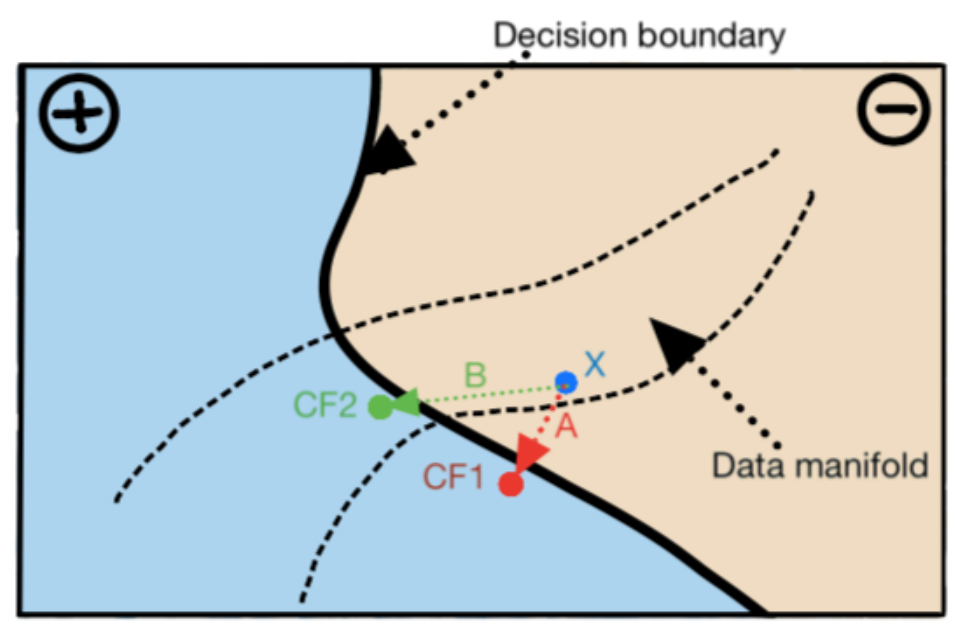
\includegraphics[width=1\textwidth]{\pathiml/figure/counterfactuals_obj}			
	\end{column}
	\begin{column}{0.6\textwidth}

\textbf{Example from \citebutton{Verma et al. (2020)}{https://arxiv.org/abs/2010.10596}} 
\begin{itemize}
    \item Two possible paths for \textcolor{blue}{$\xv$},			originally classified to $\pmb{\circleddash}$
    \item Two valid CEs in class $\pmb\oplus$: {\color{red} CF1} and {\color{green} CF2}
    \item {\color{red} Path \textbf{A} for CF1} is shorter
    \item {\color{green} Path \textbf{B} for CF2} is longer but adheres to data manifold
\end{itemize}
%Two possible paths for \textcolor{blue}{$\xv$},			originally classified in the negative class. The two counterfactuals (\textcolor{red}{CF1} and \textcolor{green}{CF2}) are valid. Note that the red path $A$ for CF1 is the shortest, whereas the green path $B$ for CF2 adheres closely to the manifold of the training data, but is longer.
\end{column}
\end{columns}
}
%\footnote[frame]{Verma et al. (2020). \href{https://arxiv.org/pdf/2010.10596.pdf}{Counterfactual Explanations for Machine Learning: A Review.}}

\end{frame}


\begin{frame}{Further Objectives}
	%\begin{itemize}
	%\item 
%For example, $o_4$ could then be the Gower distance of $\xv'$ to the nearest data point of the training dataset $\xv^{[1]}$

To ensure plausibility, $o_4$ could, e.g., be the Gower distance of $\xv'$ to its nearest data point of the training dataset which we denote $\xv^{[1]}$:
	
$$o_4(\xv', \Xmat) = \Gower(\xv', \xv^{[1]}) = \frac{1}{p} \sum_{j = 1}^{p}  \delta_G(x_j', x^{[1]}_j)$$
%\end{itemize}

We can extend the previous optimization problem by adding $o_s$ (for sparsity) and $o_4$ (for plausibility):

$$\argmin_{\xv'} \lambda_1 o_p(\fh(\xv'), y') + \lambda_2 o_f(\xv', \xv) + \lambda_3 o_s(\xv', \xv) + \lambda_4 o_4(\xv', \Xmat)$$

\end{frame}


\begin{frame}{Remarks: The Rashomon Effect}
%The solution to the optimization problem might not be unique, there can be many equally close inputs that obtain the desired classification. Correspondingly, there can be many different equally good explanations for the same decision. This is called the \textbf{Rashomon effect}.

\textbf{Issue (\textbf{Rashomon effect}):}
\begin{itemize}
    \item Solution to the optimization problem might not be unique
    \item Many equally close CE might exist that obtain the desired prediction\\
    $\Rightarrow$ Many different equally good explanations for the same decision exist
\end{itemize}

\lz\pause

\textbf{Possible solutions:}
	\begin{itemize}
	\item Present all CEs for a given $\xv$ (but: time and human processing capacity is limited)
		%\item We could present all CEs for a given case; however, time is limited and so is the human processing capacity
		%\item Another solution is to focus on one or few CEs; however, by which criterion should they be selected?
		\item Focus on one or few CEs (but: by which criterion should they be selected?)
	\end{itemize}
	
\lz\pause

\textbf{Note:}
	\begin{itemize}
        \item As the model is generally non-linear, inconsistent and diverse CEs can arise\\
        e.g. suggesting either an increase or decrease in credit duration (confuses the explainee)
		\item How to deal with the Rashomon effect is considered an open problem in IML
	\end{itemize}
\end{frame}

\begin{frame}[c]{Remarks: Model or Real-World}

	\begin{itemize}[<+->]
	\item Most CEs provide explanations of model predictions, but CEs might appear to explain the real-world for end-users\\
$\leadsto$ Transfer of model explanations to explain real-world is generally not permitted
	\item Consider a CE that proposes to increase the feature age by 5 to obtain the loan\\
	$\leadsto$ a loan applicant takes this information and applies 5 years later for the loan
	\item However, by then, many 
	%of their 
	other feature values 
	%properties 
	might have changed\\
	$\leadsto$ not only age, also other causally dependent features e.g. job status might have changed \\%after 5 years% since they are causally dependent on age like income or the job status
	$\leadsto$ \citebutton{Karimi et al. (2020)}{https://arxiv.org/abs/2002.06278} avoid this by considering causal dependencies between features
	\item Also, the bank's algorithm might change and previous CEs are not applicable anymore
	%\item Even worse, the user might have typos in the application and in fact no changes are necessary to obtain the loan.
%		\item Actionability: We could further strengthen above's plausibility criterion by requiring counterfactuals that do not change immutable features (e.g., race, city of birth, sex). Therefore, we could  search for counterfactuals only among a defined feasible set of counterfactuals $\mathcal{A}$.
%		\item Causality: We could also restrict the search to counterfactuals that maintain any known causal relations. In the real world, if one feature is changed it affects also other features. E.g., better skills lead to better salary, but also a higher age due to the necessary training.
	\end{itemize}
%\footnote[frame]{Karimi et al. (2021). Algorithmic Recourse: From Counterfactual Explanations to Interventions.  Proceedings of the 2021 ACM Conference on Fairness, Accountability, and Transparency. 353–362.}
\end{frame}


%\endlecture

\renewcommand{\titlefigure}{\pathiml/figure/counterfactuals_heat.png}
    \renewcommand{\learninggoals}{
    	\item See two strategies to generate CEs
    	\item Know problems and limitations of CEs}
	
	\lecturechapter{Methods \& Discussion of Counterfactual Explanations}
	%\lecture{Interpretable Machine Learning}
	\mysectionslide
	
	% ------------------------------------------------------------------------------


\begin{frame}{Overview of Methods}
	Currently, multiple methods exist to calculate counterfactuals. They mainly differ in: 
	\begin{itemize}[<+->]
		\item \textbf{Targets:} Most methods focus on classification models, only few cover regression models\\
		$\leadsto$ so far, all methods remain in the supervised learning paradigm
		\item \textbf{Data:} Methods mainly focus on tabular data, few on visual/text data, none on audio data
		\item \textbf{Feature space:} Some methods can only handle numerical features, few can process mixed (numerical and discrete) feature spaces
		\item \textbf{Objectives:} Many methods focus on action guidance, plausibility and sparsity, few on other objectives like fairness or individual preferences
		\item \textbf{Model access:} Methods either require access to complete model internals, access to gradients, or only to prediction functions $\Rightarrow$ Model-agnostic and model-specific methods exist
		\item \textbf{Optimization tool:} Gradient-based algorithms (only for differentiable models), mixed-integer programming (only linear), or gradient-free algorithms e.g. Nelder-Mead, genetic algorithm
		\item \textbf{Rashomon Effect:} Many methods return a single counterfactual per run, some multiple counterfactuals, others prioritize CEs or let the user choose
	\end{itemize}
\end{frame}

\begin{frame}{First Optimization Method \citebutton{Wachter et. al (2018)}{http://dx.doi.org/10.2139/ssrn.3063289}}
Introduced counterfactual explanations in the context of ML predictions by solving
		\begin{equation}
			\argmin_{\xv'} \max_{\lambda} \lambda \underbrace{(\fh(\xv') - y')^2}_{o_p(\fh(\xv'), y')} + \underbrace{\sum\nolimits_{j = 1}^p |x'_j - x_j|/MAD_j}_{o_f(\xv', \xv)}
			%\label{eq:wachter}
		\end{equation}
	$MAD_j$ is the median absolute deviation of feature $j$. In each iteration, optimizers like Nelder-Mead solve the equation for $\xv'$ and then $\lambda$ is increased until a sufficiently close solution is found \\[0.2cm]
	
	%\pause
	
	This optimization problem has several shortcomings: 	
	\begin{itemize}%[<+->]
		\item We do not know how to choose $\lambda$ a priori 
		\item Due to the maximization of $\lambda$, we focus primarily on the minimization of $o_p$\\
		$\leadsto$ only if $\fh(\xv') = y'$, we focus on minimizing $o_f$ 
		\item Definition of $o_f$ only covers numerical features 
		\item Other objectives such as sparsity and plausibility of counterfactuals are neglected
	\end{itemize}
	


	%\footnote[frame]{Wachter S, Mittelstadt B, Russel C (2017). Counterfactual Explanations Without Opening the Black Box: Automated Decisions and the GDPR. Harvard Journal of Law \& Technology, 31 (2), 2018. \url{http://dx.doi.org/10.2139/ssrn.3063289}}
\end{frame}

\begin{frame}{Multi-Objective Counterfactual Explanations \citebutton{Dandl et al. (2020)}{https://arxiv.org/abs/2004.11165}}
	\begin{itemize}
		\item \textbf{Multi-Objective Counterfactual Explanations (MOC):} Instead of collapsing objectives into a single objective, we could optimize all four objectives simultaneously
	$$	\argmin_{\xv'} \left(o_p(\fh(\xv'), y'), o_f(\xv', \xv), o_s(\xv', \xv), o_4(\xv', \Xmat) \right). $$
		
		\item Note that weighting parameters like $\lambda$ are not necessary anymore
		%\item This approach is called Multi-Objective Counterfactual Explanations (MOC) and was developed by Dandl et al. in 2020. 
		\item Uses an adjusted multi-objective genetic algorithm (NSGA-II) to produce a set of diverse counterfactuals for mixed discrete and continuous feature spaces
		\item Instead of one, MOC returns multiple counterfactuals that represents different trade-offs between the objectives and are constructed to be diverse in feature space
	\end{itemize}

	%\footnote[frame]{Dandl et al. (2020) Multi-Objective Counterfactual Explanations. In: Bäck T. et al. (eds) Parallel Problem Solving from Nature – PPSN XVI. PPSN 2020. Lecture Notes in Computer Science, vol 12269. Springer, Cham.}
\end{frame}

\begin{frame}{Example: Credit Data}
	\begin{itemize}
		\item Model: SVM with RBF kernel
		\item $\xv$: First data point of credit data with $\P(y = good)  = 0.34$ of being a ``good" customer
		\item Goal: Increase the probability to $[0.5, 1]$
		\item MOC (with default parameters) found 69 CEs after 200 iterations that met the target
		\item All counterfactuals proposed changes to credit duration and many of them to credit amount
	\end{itemize}
	
	\pause
	\bigskip

    \textbf{Original observation:}\\
	\begin{table}[ht]
		\centering
		\scriptsize
		\begin{tabular}{rlrlllrrlr}
			\hline
			age & sex & job & housing & saving & checking & credit.amount & duration & purpose & $\hat{y}$ \\ 
			\hline
			 22 & female &   2 & own & little & moderate & 5951 &  48 & radio/TV & 0.34 \\ 
			\hline
		\end{tabular}
	\end{table}
	
	\pause
	\bigskip

    \textbf{Selected counterfactuals:}\\
	\begin{table}[ht]
		\centering
		\scriptsize
		\begin{tabular}{rlrlllrrlr}
			\hline
			age & sex & job & housing & saving & checking & credit.amount & duration & purpose & $\hat{y}$ \\ 
			 \hline
			 22 & female &   2 & own & little & moderate & 5951 & \cellcolor{yellow} 30 & radio/TV & 0.54 \\ 
			 22 & female &   2 & own & little & moderate & \cellcolor{yellow} 2656 & \cellcolor{yellow} 24 & radio/TV & 0.63 \\ 
			 22 & female &   2 & own & little & moderate & \cellcolor{yellow} 1454 &  \cellcolor{yellow} 12 & radio/TV & 0.72 \\ 
			\hline
		\end{tabular}
	\end{table}
\end{frame}

\begin{frame}{Example: Credit Data \citebutton{Dandl et al. (2020)}{https://arxiv.org/abs/2004.11165}}
\begin{itemize}
	\item<1-> We can visualize feature changes with a parallel plot and 2-dim surface plot
		\item<1-> Parallel plot reveals that all counterfactuals had values equal to or smaller than the values of $\xv$
		\item<2-> Surface plot illustrates why these feature changes are recommended 
		\item<2-> Counterfactuals in the lower left corner seem to be in a less favorable region far from $\xv$, but they are in high density areas close to training samples (indicated by histograms)
	\end{itemize}
	\begin{columns}\only<1->{
	\begin{column}{0.5\textwidth}  
	\centering
			%\begin{center}
		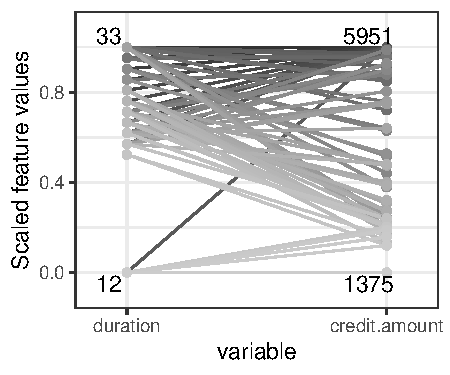
\includegraphics[width=0.75\textwidth]{\pathiml/figure/counterfactuals_credit_parallel}\\
			%\end{center}
		%\vspace{-0.2cm}
			\scriptsize{\textbf{Parallel plot:} Grey lines show feature values of CEs $\xv'$, blue line are values of $\xv$. Features without proposed changes are omitted. Bold numbers refer to range of numeric features.} 
			
		\end{column}}
		\visible<2->{
		\begin{column}{0.5\textwidth}
			%\begin{center}
			\centering
			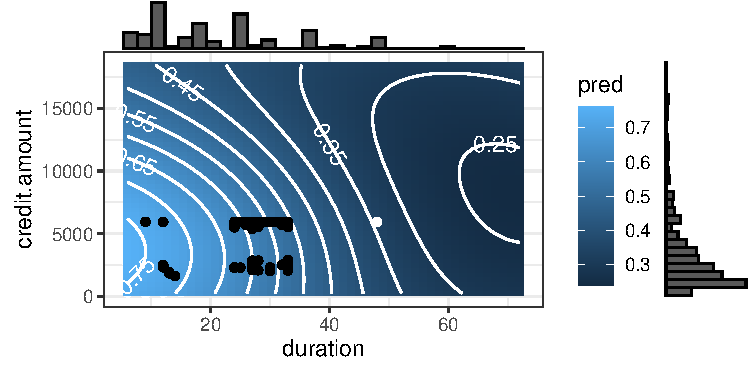
\includegraphics[width=\textwidth]{\pathiml/figure/counterfactuals_credit_heat}\\
			%\end{center}
		%\vspace{-0.2cm}
			\scriptsize{\textbf{Surface plot:} White dot is $\xv$, black dots are CEs $\xv'$. \\
			Histograms show marginal distribution of training data $\Xmat$.} 
		\end{column}
		}
	\end{columns}
%\footnote[frame]{Dandl S., Molnar C., Binder M., Bischl B. (2020) Multi-Objective Counterfactual Explanations. In: Bäck T. et al. (eds) Parallel Problem Solving from Nature – PPSN XVI. PPSN 2020. Lecture Notes in Computer Science, vol 12269. Springer, Cham.}
\end{frame}


%\begin{frame}{Example: Bike Sharing Dataset}
%	\begin{itemize}
%		\item Model: Random Forest with 500 trees
%		\item $\xv$ is the first data point of the dataset with $\fh(\xv) = 1767.93$ rental bikes. 
%		\item Our desired goal is to increase the count of total rental bikes to $y' = [3000, \infty[$
%		\item MOC (with default parameters) found 56 counterfactuals after 200 iterations that met the target.
%		\item Most counterfactuals proposed to decrease the humidity (94.6 \%) and more than half to increase the temperature (55.4\%). 
%		\item Some counterfactuals proposed additional changes to the year (2012 instead of 2011) and month (December instead of Januar).
%		\framebreak 
%		\item We can visualize feature changes with a parallel plot. 
%		\item For humidity and temperature, we can additionally show a 2-dim surface plot. 
%	\end{itemize}
%	\vspace{-0.5cm}
%	\begin{columns}
%		\begin{column}{0.5\textwidth}
%			\begin{center}
%				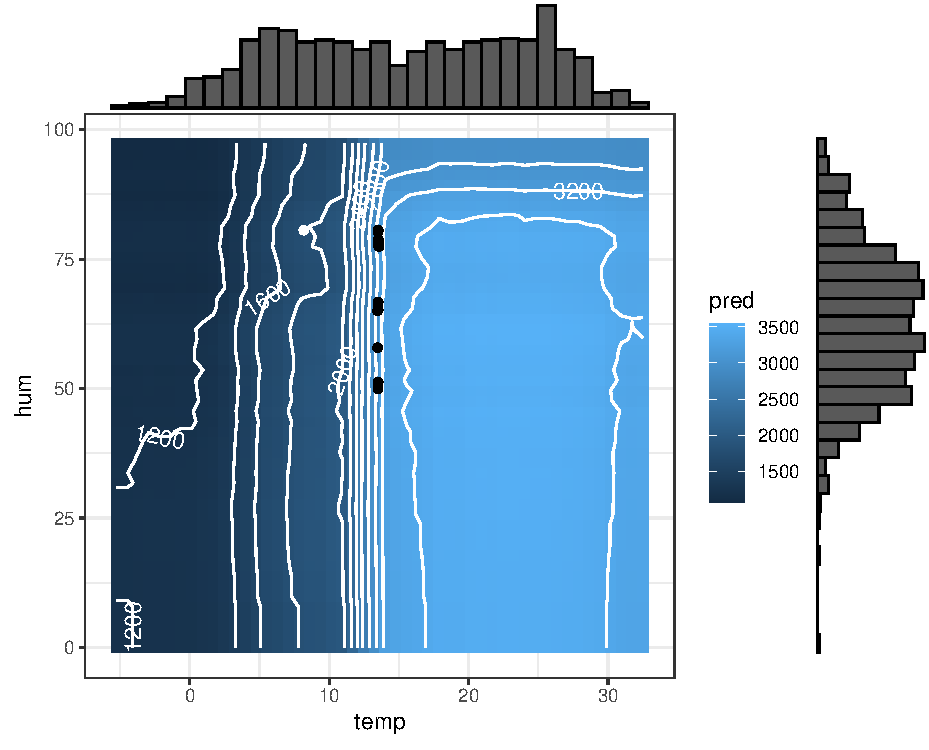
\includegraphics[width=1\textwidth]{\pathiml/figure/counterfactuals_bike_sp}
%			\end{center}
%		
%			\scriptsize{\textbf{Figure:} Response surface plot. 
%				The white dot is $\xv$, black dots are $\xv'$. The histograms display the marginal distribution of the training data $\Xmat$.} 
%				
%		\end{column}
%		\begin{column}{0.5\textwidth}  
%			\begin{center}
%				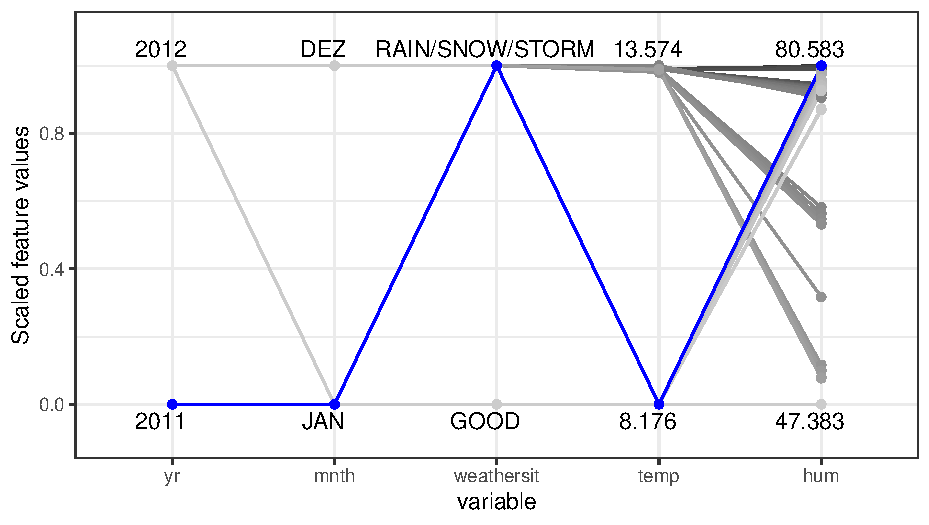
\includegraphics[width=1\textwidth]{\pathiml/figure/counterfactuals_bike_para}
%			\end{center}
%		
%		\scriptsize{\textbf{Figure:} Parallel plot. 
%			The grey lines show the feature values of the counterfactuals $\xv'$, the blue line corresponds to the values of $\xv$. Features without proposed changes are omitted. The bold numbers give minima and minima of numeric features while character strings indicate categories of character features.} 
%		
%		\end{column}
%	\end{columns}
%\end{frame}

\begin{frame}{Problems, Pitfalls, \& Limitations}
\begin{itemize}[<+->]
    \item \textbf{Illusion of model understanding:} 
    CEs explain ML decisions by pointing to few specific alternatives which reduces complexity, but is limited in explanatory power\\
    $\leadsto$ %psychologists showed that even though the perceived model-understanding of end-users increases, the objective model-understanding remained unchanged
    Psychologists have shown that although perceived model understanding of end-users increases, the objective model understanding remains unchanged
    
    %\item \textbf{Finding the right metric:} Similarity is the crucial concept for finding good CEs. However, our concept of similarity is context and domain dependent. E.g. while L1 can be a reasonable notion for tabular data, it is counterintuitive for image data. Sparsity is often desirable for end-users but not for data scientists searching for biases in the model.
    \item \textbf{Right metric:} Similarity measures are crucial to find good CEs (depends on context/domain)\\
    $\leadsto$ e.g., $L_1$ can be reasonable for tabular data but not for image data\\
    $\leadsto$ sparsity can be desirable for end-users but not for data scientists searching for model bias

    %\item \textbf{Confusing Model and Real-World:} Explanations of the model do not easily transfer to the process in which a model is applied. This information should be conveyed to the end-user.
    \item \textbf{Confusing Model and Real-World:} Model explanations are not easily transferable to reality\\
    $\leadsto$ End-users need to be aware that CE provide insights into a model not the real world %models are only approximations %This information should be conveyed to the end-user
    \item \textbf{Disclosing too much information:} \\
    CEs can reveal too much information about the model and help potential attackers
    \end{itemize}
\end{frame}

\begin{frame}{Problems, Pitfalls, \& Limitations}
\begin{itemize}[<+->]
    \item \textbf{Rashomon effect:} One, few, all? Which CEs should be shown to the end-user?\\
    $\leadsto$ No perfect solution, depends on end-users computational resources and knowledge
    \item \textbf{Actionability vs. fairness:} Some authors suggest to focus only on the actionability of CEs\\
    $\leadsto$ Counteract contestability, e.g., if ethnicity is not changed in a CE since it is not actionable, this could hide racial biases in the model
    \item \textbf{Assumption of constant model:} To provide guidance for the future, CEs assume that their underlying model does not change in the future\\
    $\leadsto$ in reality this assumption is often violated and CEs are not reliable anymore 
    \item \textbf{Attacking CEs:} Researchers can create models with great performance, which generate arbitrary explanations specified by the ML developer\\
    $\leadsto$ how faithful are CEs to the models underlying mechanism?
\end{itemize}

%	\textbf{Pitfall 3:} Rashomon Effect
%	\begin{itemize}
%		\item Due to the Rashomon Effect, multiple counterfactual explanations could be found for an instance. 
%		\item If all counterfactuals are reported the user could be overwhelmed. Instead of a comprehensible explanations for a prediction, users received an even more complex explanations.
%		\item Another option is to only report the ``best" ones. But this requires a notion for ``superiority".  
%		\item Furthermore, users might not be interested in the ``best" but most ``diverse" counterfactuals.
%		\item The best option might be to report all counterfactuals but let the user decide which one to select, e.g., based on their previous knowledge. 
%	\end{itemize}
%	\textbf{Pitfall 4:} 
%	\begin{itemize}
%		\item 
%	\end{itemize}
%	\textbf{Pitfall 5:} Confusing model explanation with real data process explanations
%	\begin{itemize}
%		\item Causal dependencies
%		\item Fixed model at time $t$ 
%		\item Wrong input by user
%	\end{itemize}
\end{frame}

%\endlecture

\endlecture

\end{document}
